\documentclass[a4paper,12pt]{book}
\usepackage{mathptmx}
\usepackage{hyperref}
\usepackage{cancel}
\usepackage{amsmath}
\usepackage{amssymb}
\usepackage{graphicx}
\usepackage{pgfplots}
\usepackage{tikz}
\usepackage{xcolor}

\author{Gábor Hadházy and Tamás Hadházy}
\title{Mathematics}
\date{\today}

\begin{document}
\maketitle

\tableofcontents

% Chapter 1 - Algebra
\chapter{Algebra and Pre-calculus}
The first chapter is about algebra. It will cover the topics that was written by Gábor Hadházy and Tamás Hadházy. Algebra and Pre-calculus are the foundation of mathematics. It is important to understand the concepts of algebra and pre-calculus before moving on to more advanced topics.

\section{Essentials}
This section will cover the essentials in order to get started. 
\subsection{The set of Real numbers}
\begin{itemize}
    \item $\mathbb{N} = \{1, 2, 3, ...\}$ - - The set of natural numbers. 
    \item $\mathbb{Z} = \{..., -2, -1, 0, 1, 2, ...\}$ - The set of integers.
    \item $\mathbb{Q} = \{\frac{a}{b} | a, b \in \mathbb{Z}, b \neq 0\}$ - The set of rational numbers. 
    \item $\mathbb{I}$ - The set of Irrational Numbers(Real numbers that are not rational). 
    \item $\mathbb{R} = \mathbb{Q} \cup \mathbb{I}$
\end{itemize}


\subsection{The properties of Real numbers}
\includegraphics[width=1.1\textwidth]{algebra-pre-calculus/algebra/essentials/properties.png}

\subsection{Addition and Subtraction}
The number 0 is special for addition; it is called the additive identity because $a+0=a$ for any real number $a$. Every real number $a$ has a negative, $-a$, that satisfies $a+(-a)=0$. Subtraction is the operation that undoes addition; to subtract a number from another, we simply add the negative of that number. By definition
$$
a-b=a+(-b)
$$
To combine real numbers involving negatives, we use the following properties.
\includegraphics[width=1.1\textwidth]{algebra-pre-calculus/algebra/essentials/properties_addition_subtraction.png}

Property 6 states the intuitive fact that $a-b$ and $b-a$ are negatives of each other. \\
Property 5 is often used with more than two terms:
$$
    -(a+b+c)=-a-b-c
$$

\subsection{Multiplication and Division}
The number 1 is special for multiplication; it is called the \textbf{multiplicative identity} because $a \cdot 1=a$ for any real number $a$. Every nonzero real number $a$ has an inverse, $1 / a$, that satisfies $a \cdot(1 / a)=1$. Division is the operation that undoes multiplication; to divide by a number, we multiply by the inverse of that number. If $b \neq 0$, then, by definition,
$$
a \div b=a \cdot \frac{1}{b}
$$
We write $a \cdot(1 / b)$ as simply $a / b$. We refer to $a / b$ as the quotient of $a$ and $b$ or as the fraction $a$ over $b$; $a$ is the numerator and $b$ is the denominator (or divisor). To combine real numbers using the operation of division, we use the following properties. \\
\includegraphics[width=1.1\textwidth]{algebra-pre-calculus/algebra/essentials/properties_multiplication_division.png}

When adding fractions with different denominators, we don’t usually use Property 4.
Instead we rewrite the fractions so that they have the smallest possible common denominator (often smaller than the product of the denominators), and then we use Property 3. This
denominator is the Least Common Denominator (LCD) described in the next example.

\subsection{Using the LCD to Add Fractions}

Evaluate: $\frac{5}{36}+\frac{7}{120}$
\textbf{Solution.} Factoring each denominator into prime factors gives
$$
36=2^2 \cdot 3^2 \quad \text { and } \quad 120=2^3 \cdot 3 \cdot 5
$$
We find the least common denominator (LCD) by forming the product of all the prime factors that occur in these factorizations, using the highest power of each prime factor. Thus the LCD is $2^3 \cdot 3^2 \cdot 5=360$. So
$$
\begin{aligned}
\frac{5}{36}+\frac{7}{120} & =\frac{5 \cdot 10}{36 \cdot 10}+\frac{7 \cdot 3}{120 \cdot 3} & \text { Use common denominator } \\
& =\frac{50}{360}+\frac{21}{360}=\frac{71}{360} & \begin{array}{l}
\text { Property } 3: \text { Adding fractions with the } \\
\text { same denominator }
\end{array}
\end{aligned}
$$

\subsection{Real line}

The real numbers can be represented by points on a line, as shown below. The
positive direction (toward the right) is indicated by an arrow. We choose an arbitrary
reference point O, called the origin, which corresponds to the real number 0. Given any
convenient unit of measurement, each positive number x is represented by the point on
the line a distance of x units to the right of the origin, and each negative number -x is
represented by the point x units to the left of the origin. The number associated with the
point P is called the coordinate of P, and the line is then called a coordinate line, or a
real number line, or simply a real line. Often we identify the point with its coordinate
and think of a number as being a point on the real line.

\begin{align*}
    \includegraphics[width=1.1\textwidth]{algebra-pre-calculus/algebra/essentials/real-line.png}
\end{align*}

\section{Absolute Value and Distance}
The absolute value of a number $a$, denoted by $|a|$ , is the distance from $a$ to 0 on
the number line. Distance is always positive or zero, so we have
$|a|\geq0$ for every number $a$. Remembering that $-a$ is positive when $a$ is negative, we have the following definition.

\begin{equation*}
    |a| = \begin{cases}
        \;a  & \textnormal{if} \ a \geq 0 \\
        \;-a & \textnormal{if} \ a < 0
    \end{cases}
\end{equation*}

(a) $|3|=3$ \\
(b) $|-3|=-(-3)=3$ \\
(c) $|0|=0$ \\
(d) $|3-\pi|=-(3-\pi)=\pi-3 \quad($ since $3<\pi \quad \Rightarrow \quad 3-\pi<0)$

\subsection{Properties of Absolute Value}
\begin{enumerate}
    \item $|a| \geq 0$
    \item $|a|=|-a|$
    \item $|a b|=|a||b|$
    \item $\displaystyle \left|\frac{a}{b}\right|=\frac{|a|}{|b|}$
    \item $|a+b| \leq|a|+|b|$
\end{enumerate}

\subsection{Distance Between Points on the Real line}

What is the distance on the real line between the numbers -2 and 11? From
Figure 11 we see that the distance is 13. We arrive at this by finding either
$ |11-(-2)|=13$ or $|(-2)-11=13|$. From this observation we make the following definition. \\

If $a$ and $b$ are real numbers, then the \textbf{distance} between the points $a$ and $b$ on the real line is: \\
$$ d(a,b)=|a-b| $$

From the Property 6 of negatives it follows that
$$ |b-a| = |a-b|$$
$$ |3-7| = |7-3| = 4 $$

This confirms that, as we would expect, the distance from a to b is the same as the
distance from b to a.

\textbf{Example.} The distance between then numbers -8 and 2 is $d(-8,2)=|-8-2|=|-10|=10$.

\subsubsection*{Exercises}
For Exercises please download the book from here(\url{https://faculty.ksu.edu.sa/sites/default/files/precalculus-mathematics_for_calculus-j._stewart_l._redlin_and_s._watson-cengage_learning_7th_edition_2015.pdf}) and you can go to the 37th page for exercises.  % Section 1 - Essentials
\section{Exponentiation}
When starting out with Exponentiation it is important first to understand the different parts of an exponential expression, so let's consider:
$$b^x = \underbrace{b \cdot b \cdot ... \cdot b}_{x \ times}$$
\begin{itemize}
  \item $b$ is the \textbf{base}.
  \item $x$ is the \textbf{exponent}.
\end{itemize}

As a reminder $ x^0 = 1 $

Let's discuss the different rules of Exponentiation:
\subsection{Product Rule}
To find the product of two exponential expression with the same base, add the exponents. 
$$ x^{n} \cdot x^{m} = x^{n+m} $$

\subsection{Quotient Rule}
When two exponential expressions with the same base are divided,  to find their quotient subtract their exponents. 
$$ \frac{x^n}{x^m} = x^{n-m} $$

\subsection{Power Rule}
When you raise an power to a power in an exponential expression to get the product, multiply the exponents
$$ (x^{n})^{m} = x^{n \cdot m} $$ 
$$ OR $$
$$ (x^{n})^{m} = \underbrace{x^n \cdot ... \cdot x^n}_{m \ times} $$
Here it is proven that the power rule is simply just the product rule.

\subsection{Negative Exponents}
When dealing with negative exponents this equation will apply: 
$$ x^{-n} = \frac{1}{x^n} $$

Since, 
$$ \frac{1}{x} = \frac{x^0}{x^1} = x^{0-1} = x^{-1} $$
It is important to note that this is just only one way of proving this, there are a couple more. 

\subsection{Fractional Exponents}
$$ \large x^{\frac{1}{n}} = \sqrt[n]{x} $$
The proof of this can be found in the next section \hyperref[sec:radicals]{Radicals(click to redirect)}.

\subsection{Additional rules}
Distribute an exponent over a product: $(x \ y)^{n} = x^{n} \ y^{n}$ \\
Distribute an exponent over a quotient: $  (\frac{a}{b})^{n} = \frac{a^{n}}{b^{n}}$

\begin{align*}
  \includegraphics[width=1.2\textwidth]{algebra-pre-calculus/algebra/exponentiation/laws-of-exponents.png}
\end{align*}

\newpage % Section 2 - Exponentiation
\label{sec:radicals}
\section{Radicals}
$$ \sqrt[n]{x} $$
\begin{itemize}
  \item $x$ is the \textbf{radicand}.
  \item $n$ is the \textbf{index}(nth root).
  \item $ \sqrt[n]{x}$ expression is the \textbf{radical}
\end{itemize}

As promised let's look at the fractional exponent equation. If $n$ is a positive integer that is greater than $1$ and a is a real number then,
$$ \sqrt[n]{a} = a^{\frac{1}{n}} $$

We are often referring the left side of the equation as the \textbf{radical form} and the right side of the equation as the \textbf{exponent form}

\subsubsection{Proof}
In order to prove this equation we can establish first this: 
$$ (a^{\frac{1}{n}})^{n} = a^{n \cdot \frac{1}{n}} = a^{\frac{n}{n}} = a $$
Let's take an example to avoid confusion: 
$$ (9^{\frac{1}{2}})^2 = 9^{\frac{1}{2} \cdot2} = 9^{\frac{2}{2}} = 9 $$

To put this into words $ 9^{\frac{1}{2}} $ is the number that when squared will return back $ 9 $. In other words this is exactly what it meant by the root(in this case square root) which will return back the number that when squared it will be 9. Therefore: 
$$ 9^{\frac{1}{2}} =  \sqrt[2]{9} = 3 $$

Since,
$$ (3)^2 = 9 = (9^{\frac{1}{2}})^2 $$

Therefore the equation has been proven: 
$$ \sqrt[n]{a} = a^{\frac{1}{n}} $$

It is very important to note a misconception here. The index is required in these radical expressions to make sure that we correctly evaluate the radical. There is one exception to this rule and that is square root.
$$ \sqrt[2]{a} = \sqrt[]{a} $$
In every other cases we \textbf{must} define the index, because otherwise it will be considered as a square root, Whenever working with square roots the index can be omitted.

\subsubsection{General rational exponent}
Since, $ a^{\frac{1}{n}} = \sqrt[n]{a} $.
Let's establish the general rational exponent in terms of radicals as follows. 
$$ a^{\frac{m}{n}} = (a^{\frac{1}{n}}) ^{m} = (\sqrt[n]{a})^m $$
$$ OR $$
$$ a^{\frac{m}{n}} = (a^m) ^{\frac{1}{n}} = \sqrt[n]{a^m} $$

Since being aware of the \textbf{Associative Property of Multiplication}, the order of the multiplication can be changed. 

Therefore, 
$$ a^{\frac{m}{n}} = \sqrt[n]{a^m} $$

\subsection{Properties of radicals}
\begin{itemize}
  \item $\sqrt[n]{a^n} = a$ \ This is simply true because when trying to find the $n$th root of a number and  also raising the number to that power then that's simply will be equal to the number.  \\
Consider this as an example,
$$ \sqrt[]{9^2} = \sqrt[]{81} = 9$$
   \item $ \sqrt[n]{ab} = \sqrt[n]{a} \sqrt[n]{b} $ \\
   To prove this consider this, \\
    1. Start with the left-hand side (LHS) of the equation,
    $ \sqrt[n]{ab} $ Using the definition of the nth root:
    $ \sqrt[n]{ab} = (ab)^{\frac{1}{n}} $ \\
    2. Next apply the product rule of exponents, which states that $ a^m \cdot a^n = a^{m+n} $ Therefore, $ (ab)^{\frac{1}{n}} = a^{\frac{1}{n}} \cdot b^{\frac{1}{n}} $ \\ 
    3. Now, rewrite the exponents as radicals:
    $ a^{\frac{1}{n}} $ is equivalent to $ \sqrt[n]{a} $ and $ b^{\frac{1}{n}} $ is equivalent to $ \sqrt[n]{b} $ \\
    4. So, we have: $ a^{\frac{1}{n}} \cdot b^{\frac{1}{n}} = \sqrt[n]{a} \cdot \sqrt[n]{b} $ \\
    5. Finally this proves that: $ \sqrt[n]{ab} = \sqrt[n]{a} \cdot \sqrt[n]{b} $
    \item $ \sqrt[n]{\frac{a}{b}} = \frac{\sqrt[n]{a}}{\sqrt[n]{b}} $ To prove this consider this, \\
    1. As previously Start with the left-hand side (LHS) of the equation: $ \sqrt[n]{\frac{a}{b}} $ \\
    2. Now using the definition of the nth root: $ \sqrt[n]{\frac{a}{b}} = \left(\frac{a}{b}\right)^{\frac{1}{n}} $ \\
    3. Apply the power rule of the exponents which states that: \\ $ (a^m)^{\frac{1}{n}} = a^{m \cdot \frac{1}{n}} = a^{\frac{m}{n}}$, Therefore when we are dealing with a fraction as the base it is the same when dealing with numbers that are not fractions: 
$$ \left(\frac{a}{b}\right)^{\frac{1}{n}} = \frac{a^{\frac{1}{n}}}{b^{\frac{1}{n}}} $$ Since, \\
$$ (\frac{a}{b})^c = \frac{a^c}{b^c} $$ \\
With an example: $ (\frac{a}{b})^2 = \frac{a}{b} \cdot \frac{a}{b} = \frac{a^2}{b^2} $ \\
	4. Now rewrite the exponents as radicals: $ a^{\frac{1}{n}} $ is equivalent to $ \sqrt[n]{a} $ and  $b^{\frac{1}{n}}$ is equivalent to $ \sqrt[n]{b} $ \\
	5. So, we have: 
	$$ \frac{a^{\frac{1}{n}}}{b^{\frac{1}{n}}} = \frac{\sqrt[n]{a}}{\sqrt[n]{b}} $$ \\
	6. Finally, this proves that: 
	$$ \sqrt[n]{\frac{a}{b}} = \frac{\sqrt[n]{a}}{\sqrt[n]{b}} $$ \\
	\\
	
	\item Also note that while we can “break up” products and quotients under a radical we can’t do the same thing for sums or differences. In other words,
	$$ \sqrt[n]{a+b} \neq \sqrt[n]{a}+ \sqrt[n]{b}  $$ 
	$$ AND $$
	$$ \sqrt[n]{a-b} \neq \sqrt[n]{a}- \sqrt[n]{b} $$ \\
These can simply be proven by examples, 
$$ 5 = \sqrt25 = \sqrt{9+16} \neq \sqrt9 + \sqrt16 = 3+4 = 7 $$

\begin{align*}
  \includegraphics[width=0.8\textwidth]{algebra-pre-calculus/algebra/radicals/properties_of_nth_roots.png}
\end{align*}

\end{itemize}
\subsection{Using the Laws of Exponents with Rational Exponents}
(a) \scalebox{1.1}{$a^{1 / 3} a^{7 / 3}=a^{8 / 3}$} $\Rightarrow$
\textbf{Law 1: $a^m a^n=a^{m+n}$} \\ \break
(b) \scalebox{1.1}{$\frac{\displaystyle a^{2 / 5} a^{7 / 5}}{a^{3 / 5}}=a^{2 / 5+7 / 5-3 / 5}=a^{6 / 5}$} $\Rightarrow$
\textbf{Law 1, Law 2:} $\frac{a^m}{a^n}=a^{m-n}$ \\ \break
(c)
$$
\begin{aligned}
\left(2 a^3 b^4\right)^{3 / 2} & =2^{3 / 2}\left(a^3\right)^{3 / 2}\left(b^4\right)^{3 / 2} \\
& =(\sqrt{2})^3 a^{3(3 / 2)} b^{4(3 / 2)} \\
& = \sqrt{2^2} \cdot \sqrt{2} \cdot a^{9 / 2} b^{6} \\
& =2 \sqrt{2} \cdot a^{9 / 2} \cdot b^6
\end{aligned}
$$
\textbf{Law 4:} $(a b c)^n=a^n b^n c^n$ \\
\textbf{Law 3:} $\left(a^m\right)^n=a^{m n}$ \\ \break
(d)
$$
\begin{aligned}
\left(\frac{2 x^{3 / 4}}{y^{1 / 3}}\right)^3 \cdot \left(\frac{y^4}{x^{-1 / 2}}\right) & =\frac{2^3\left(x^{3 / 4}\right)^3}{\left(y^{1 / 3}\right)^3} \cdot\left(y^4 x^{1 / 2}\right) \\
& =\frac{8 x^{9 / 4}}{y} \cdot y^4 x^{1 / 2} \\
& =8 x^{11 / 4} y^3
\end{aligned}
$$
\textbf{Laws 5, 4, and 7 \\
Law 3 \\
Laws 1 and 2}

\subsection{Simplifying by Writing Radicals as Rational Exponents}
\textbf{(a)} $\displaystyle \frac{1}{\sqrt[3]{x^4}}=\frac{1}{x^{4 / 3}}=x^{-4 / 3} \Rightarrow$ Definition of rational and negative exponents \\ \break
\textbf{(b)} $(2 \sqrt{x})(3 \sqrt[3]{x})=\left(2 x^{1 / 2}\right)\left(3 x^{1 / 3}\right)$ $=6 x^{1 / 2+1 / 3}=6 x^{5 / 6} \Rightarrow$ Definition of rational exponents \\ \break 
\textbf{(c)}
$$
\begin{aligned}
\sqrt{x \sqrt{x}} & =\left(x x^{1 / 2}\right)^{1 / 2} \\
& =\left(x^{3 / 2}\right)^{1 / 2} \\
& =x^{3 / 4}
\end{aligned}
$$

\textbf{Law 1}
\textbf{Definition of rational exponents} \\
\textbf{Law 1} \\
\textbf{Law 3} \\

\subsection{Rationalizing the Denominator; Standard Form}
It is often useful to eliminate the radical in a denominator by multiplying both numerator and denominator by an appropriate expression. This procedure is called \textbf{rationalizing the denominator}. If the denominator is of the form $\sqrt{a}$, we multiply numerator
and denominator by $\sqrt{a}$. In doing this we multiply the given quantity by 1, so we do
not change its value. For instance,

$$
\displaystyle \frac{1}{\sqrt{a}}=\frac{1}{\sqrt{a}} \cdot 1=\frac{1}{\sqrt{a}} \cdot \frac{\sqrt{a}}{\sqrt{a}}=\frac{\sqrt{a}}{a}
$$
Note that the denominator in the last fraction contains no radical. In general, if the denominator is of the form $\sqrt[n]{a^m}$ with $m<n$, then multiplying the numerator and denominator by $\sqrt[n]{a^{n-m}}$ will rationalize the denominator, because (for $a>0$ )

\begin{align*}
  \scalebox{1.3}{$
\displaystyle \sqrt[n]{a^m} \sqrt[n]{a^{n-m}}=\sqrt[n]{a^{m+n-m}}=\sqrt[n]{a^n}=a
$}
\end{align*}

The idea behind this is that when you subtract $n-m$ what you are doing is looking for the number that when you add with $m$ you are going to get $n$ and by doing so, whenever you have $\sqrt[n]{a^m} \sqrt[n]{a^{n-m}}$ this part since you have the same base you can just add the exponents up like this: $ \sqrt[n]{a^{m+n-m}} $ and since $ m+n-m = n $ then you will have $ \sqrt[n]{a^n} $ and since the $ n $th root and the $ n $th power cancel each other out you will be left with $ a $.

With an example, let's say that we have $a=4$ and $n=3$ and $m=1$ then we have:
$$ \sqrt[3]{4^1} \sqrt[3]{4^{3-1}} = \sqrt[3]{4^1} \sqrt[3]{4^2} = \sqrt[3]{4^3} = 4 $$
When we have subtracted $ 3-1 $ we have found the number that when we add with $ 1 $ we will get $ 3 $ and that number is $ 2 $ and since we have the same base we can just add the exponents up and we will get $ 3 $ and since the $ 3 $rd root and the $ 3 $rd power cancel each other out we will be left with $ 4 $. 
In conclusion we are always trying to find the number that when we add with $ m $ we will get $ n $ and that number is $ n-m $ and since we have the same base we can just add the exponents up and we will get $ n $ and since the $ n $th root and the $ n $th power cancel each other out we will be left with $ a $. 

\subsubsection{Examples of Rationalizing the Denominator}
Put each fractional expression into Standard form by rationalizing the denominator. \\
\textbf{(a)} $\displaystyle \frac{2}{\sqrt{3}}=\frac{2}{\sqrt{3}} \cdot \frac{\sqrt{3}}{\sqrt{3}}=\frac{2\sqrt{3}}{\sqrt{3\cdot3}}=\frac{2\sqrt{3}}{\sqrt{9}}=\frac{2\sqrt{3}}{3}$ \\ 
Here we have multiplied numerator and denominator by $\sqrt{3}$, which is the denominator of the given fraction. By doing so we got rid of the radical in the denominator. \\
\textbf{(b)} $\displaystyle \frac{1}{\sqrt[3]{5}}=\frac{1}{\sqrt[3]{5}} \cdot \frac{\sqrt[3]{5^2}}{\sqrt[3]{5^2}}=\frac{\sqrt[3]{5^2}}{\sqrt[3]{5\cdot5^2}}=\frac{\sqrt[3]{5^2}}{\sqrt[3]{5^3}}=\frac{\sqrt[3]{25}}{5}$ \\
Here we have multiplied numerator and denominator by $\sqrt[3]{5^2}$, the reason why is because when we are dealing with a cube root we are looking for the number that when we add with $ 1 $(which comes from the $5$'s exponent  $\sqrt[3]{5}$) we will get $ 3 $ and that number is $ 2 $ so that's why $\sqrt[3]{5^2}$, and since we have the same base we can just add the exponents up and we will get $ 3 $. and since the $ 3 $rd root and the $ 3 $rd power cancel each other out we will be left with $ 5 $. \\
\textbf{(c)} $\displaystyle \sqrt[7]{\frac{1}{a^2}} = \frac{1}{\sqrt[7]{a^2}} = \frac{1}{\sqrt[7]{a^2}} \cdot \frac{\sqrt[7]{a^5}}{\sqrt[7]{a^5}} = \frac{\sqrt[7]{a^5}}{\sqrt[7]{a^7}} = \frac{\sqrt[7]{a^5}}{a}$ \\
Here we have multiplied numerator and denominator by $\sqrt[7]{a^5}$, the reason why is because when we are dealing with a $ 7 $th root we are looking for the number that when we add with $ 2 $(which comes from the $a$'s exponent in $a^2$) we will get $ 7 $ and that number is $ 5 $ so that's why $\sqrt[7]{a^5}$, and since we have the same base we can just add the exponents up and we will get $ 7 $. and since the $ 7 $th root and the $ 7 $th power cancel each other out we will be left with $ a $. \\ % Section 3 - Radicals
\section{Algebraic Expressions}
A \textbf{variable} is a letter that can represent any number from a given set of numbers. If we
start with variables, such as $x$, $y$, and $z$, and some real numbers and combine them using
addition, subtraction, multiplication, division, powers, and roots, we obtain an \textbf{algebraic expression}. Here are some examples:

$$ 
    2x^2-3x+4 \quad \sqrt{x}+10 \quad \frac{y-2z}{y^2+4}
$$

A \textbf{monomial} is an expression of the form $ax^k$
, where a is a real number and k is a
nonnegative integer. A \textbf{binomial} is a sum of two monomials and a \textbf{trinomial} is a sum
of three monomials. In general, a sum of monomials is called a \textbf{polynomial}. For example, the first expression listed above is a polynomial, but the other two are not.

\begin{align*}
    \includegraphics[width=1.1\textwidth]{algebra-pre-calculus/algebra/algebraic-expressions/polynomial definition.png}
\end{align*} \break

Note that the degree of a polynomial is the highest power of the variable that appears
in the polynomial.


\begin{align*}
    \includegraphics[width=1.1\textwidth]{algebra-pre-calculus/algebra/algebraic-expressions/algebraic-expression-spreadsheet.png}
\end{align*} \break

We add and subtract polynomials using the properties of real numbers that were discussed earlier. The idea is to combine like terms (that is, terms with the same
variables raised to the same powers) using the Distributive Property. For instance,

$$ 
    5x^7+3x^7-2x^7 = (5+3-2)x^7 = 6x^7
$$

But we already know this. 

To find the product of polynomials or other algebraic expressions, we need to use the
Distributive Property repeatedly. In particular, using it three times on the product of two
binomials, we get

$$ 
    (a+b)(c+d) = a(c+d)+b(c+d) = ac+ad+bc+bd
$$

\subsection{Special Product Formulas}
Certain types of products occur so frequently that you should memorize them. You can
verify the following formulas by performing the multiplications.

\begin{align*}
    \includegraphics[width=1.1\textwidth]{algebra-pre-calculus/algebra/algebraic-expressions/special_product_formulas.png}
\end{align*} \break

\subsection{Factoring Common Factors}
We use the Distributive Property to expand algebraic expressions. We sometimes need
to reverse this process (again using the Distributive Property) by factoring an expression as a product of simpler ones.
For example,
\begin{align*}
    &A. \quad 15 + 25x = 5(3 + 5x) \\
    &B. \quad x^2y + y^2x^3 = x^2y(1 + xy) \\
\end{align*}
You can always check whether you have factored correctly by expanding the brackets.

\subsection{Factoring quadratics}
A quadratic is an expression with a squared term, then just a term with a variable, then a constant. 
\\ Like this: $ax^2 + bx + c$ 
More about solving quadratic equations and quadratic equations in general can be found in the next section \hyperref[sec:quadratic-equations]{Quadratic Equations(click to redirect)}.


We are looking for two numbers that multiply you get $c$ and when you add them you get $b$.
The reason why: 
$$ (x + m)(x + n) = \\ x^2 + mx + nx + mn = x^2 + \underbrace{(m + n)}_b x + \underbrace{(mn)}_c $$

$m$ and $n$ are the two numbers we are looking for. As you can see $m + n = b$ and $mn = c$. \\

\textbf{Example}. Factor $x^2 - 6x + 8$ \\
We are looking for two numbers that multiply you get $8$ and when you add them you get $-6$. \\
The two numbers are $-2$ and $-4$ because $-2 \cdot -4 = 8$ and $-2 + -4 = -6$. \\
Therefore, 
\begin{align*}
    x^2 - 6x + 8 &= (x - 2)(x - 4) \\
\end{align*}

\textbf{Example}. Factor $10x^2 + 11x - 6$ \\
\begin{itemize}
    \item Step 1. Multiply the leading coefficient (10) and the constant term (-6) to get -60. \\
    \textbf{Why?} The main goal in factoring a quadratic equation is to express it as the product of two binomials(like (2x+4)(4x+5)). 
    In the case of a quadratic with a leading coefficient (the coefficient of $x^2$) not equal to 1, like $10x^2$ in our example, we need to find two binomials of the form $(ax + b)(cx + d)$ e.g $(2x + 4)(5x+2)$ such that their product equals the given quadratic. 
    So, in this context, we are essentially trying to break down the original quadratic ($10x^2 - 11x - 6$) into two binomials, and we start by looking for two numbers that will help us achieve this. These two numbers should meet two criteria:
    \begin{itemize}
        \item Their product should equal the product of the leading coefficient and the constant term (in this case, $10 \cdot -6 = -60$).
        \item Their sum should equal the coefficient of the x-term (in this case, -11)
    \end{itemize}
    By finding such numbers, we can rewrite the middle term of the quadratic equation (the -11x term) as the sum or difference of two terms, each of which can be factored more easily. This allows us to perform factoring by grouping, making the overall factoring process more manageable.
    \item Step 2.  Find two numbers that multiply to -60 and add up to the coefficient of the x-term (-11). In this case, those two numbers are -15 and 4 because $(-15) \cdot 4 = -60$ and $(-15) + 4 = -11$.
    \item Step 3. Rewrite the middle term (-11x) using the two numbers found in step 2: 
    $$ 10x^2 - 15x + 4x - 6 $$
    \item Step 4. Group the terms: Group the first two terms $(10x^2 - 15x)$ and the last two terms $(4x - 6)$. This will gve us: 
    $$ 5x(2x - 3) + 2(2x - 3) $$
    \item Step 5. Factor out the HCF of each group: 
    $$ 5x(2x - 3) + 2(2x - 3) = (5x + 2)(2x - 3) $$

\end{itemize}
And we are done factorising the quadratic equation.

\subsection{Difference of squares}
The difference of squares is a squared term minus another squared term.
\\ Like this: $a^2 - b^2 = (a+b)(a-b) = a^2-ab+ab-b^2 $ 

\textbf{Example.} Factor $x^2 - 9$ 
$$ (x+3)(x-3) $$


\textbf{Example.} Factor $9p^2 - 1$ 
$$ (3p+1)(3p-1) $$

\subsection{Difference or sum of cubes}
The difference or sum of cubes is a cubed term plus or minus another cubed term.

$$ a^3 - b^3 = (a-b)(a^2+ab+b^2) $$ Because, $$(a-b)(a^2+ab+b^2) = a^3 - ab^2 + a^2b - ab^2 + b^3 = a^3 - 2ab^2 + b^3 $$ 

And, 
$$ a^3 + b^3 = (a+b)(a^2-ab+b^2) $$ Because, $$(a+b)(a^2-ab+b^2) = a^3 + ab^2 - a^2b + ab^2 + b^3 = a^3 + 2ab^2 + b^3 $$ 
\\
\textbf{Example.} Factor $x^3 - 8$ \\
We know that $x^3 - 8 = x^3 - 2^3$
Therefore,
$$ (x-2)(x^2+2x+4) $$

if we expand out: 
$$ (x-2)(x^2+2x+4) = x^3 + 2x^2 + 4x - 2x^2 - 4x - 8 = x^3 - 8 $$
Therefore our answer is correct.

\subsection{Additional examples of factoring}
\textbf{Example.} Which of these expressions DOES NOT factorise?

A. $x^2 + x$ \\
This can be factored by pulling out the highest common factor. \\
$$ x^2 + x = x(x+1) $$

B. $x^2 - 25$ \\
This also can be factored by difference of squares. \\
$$ x^2 - 25 = (x+5)(x-5) $$

C. $x^2 + 4$ \\
This cannot be factored because it is a sum of squares not a difference of squares. \\

D. $x^3+2x^2+3x+6$ \\
This can also be factored by grouping. \\
$$ x^3+2x^2+3x+6 = x^2(x+2)+3(x+2) = (x^2+3)(x+2) $$

E. $5x^2-14x+8$ \\
This can also be factored by using the method of factoring quadratics when $a \neq 1$. \\
Therefore we can multiply the leading coefficient (5) and the constant term (8) to get 40. \\
We are looking for two numbers that multiply you get 40 and when you add them you get -14 and those are -10 and -4. \\
So we can rewrite the middle term (-14x) using the two numbers found:
$$ 5x^2 - 10x - 4x + 8 $$ 
Then we can group them together:
$$ 5x(x - 2) - 4(x - 2) $$
And finally factor out the HCF of each group:
$$ (5x - 4)(x - 2) $$

Eventually the answer for our question is C. $x^2 + 4$ because it cannot be factored.

\subsection{Tips and Extra examples}
\begin{itemize}
    \item Always look for the highest common factor first. That will simplify things and make the rest of the factoring more easier. 
    \item You might need to do several steps of factoring to get the final answer. For example you might have to pull out the HCF first then you can do factoring by grouping or factoring quadratics. Then you might also apply difference of squares or difference or sum of cubes. Keep factoring as far as you can go.
\end{itemize}

\textbf{Extra Example} Factor $2z^2 + 3z -14$ \\
Again as previously done first we need to multiply the leading coefficient (2) and the constant term (-14) to get -28. \\ 
We are looking for two numbers that multiply you get -28 and when you add them you get 3 and those are 7 and -4. \\
So we can rewrite the middle term (3z) using the two numbers found:
$$ 2z^2 + 7z - 4z - 14 $$ 
Then we can group them together:
$$ z(2z + 7) - 2(2z + 7) $$
And finally factor out the HCF of each group:
$$ (z - 2)(2z + 7) $$

\textbf{Extra Example} Factor $-5v^2-45v+50$ \\
Again as previously done first we need to multiply the leading coefficient (-5) and the constant term (50) to get -250. \\
We are looking for two numbers that multiply you get -250 and when you add them you get -45 and those are -50 and 5. \\
So we can rewrite the middle term (-45v) using the two numbers found:
$$ -5v^2 - 50v + 5v + 50 $$ 
Then we can group them together:
$$ -5v(v + 10) + 5(v + 10) $$
And finally factor out the HCF of each group:
$$ (-5v + 5)(v + 10) $$
This can be further simplified to:
$$ -5(v - 1)(v + 10) $$
Another solution for this could have been that first we could have pulled out the HCF which is -5 and then we could have factored the quadratic. \\
$$ -5v^2 - 45v + 50 = -5(v^2 + 9v - 10) $$
And this is really easy since $ a = 1 $ Therefore we need two numbers that multiply you get -10 and when you add them you get 9 and those are 10 and -1. \\
So we can say that: 
$$ -5(v^2 + 9v - 10) = -5(v + 10)(v - 1) $$

\subsection{Special Factoring Formulas}
\begin{align*}
    \includegraphics[width=1.1\textwidth]{algebra-pre-calculus/algebra/algebraic-expressions/special_factoring_formulas.png}
\end{align*} \break

When we factor an expression, the result can sometimes be factored further. In general, we first factor out common factors, then inspect the result to see whether it can be
factored by any of the other methods of this section. We repeat this process until we
have factored the expression completely

\subsection{Factoring Expressions with Fractional Exponents}
Factor each expresson. \\ \break
\textbf{(a)} \scalebox{1.2}{$3x^{\frac{3}{2}}-9x^{\frac{1}{2}}+6x^{-\frac{1}{2}}$ = $3x^{-\frac{1}{2}}(x^2-3x+2)$ = $3x^{-\frac{1}{2}}(x-2)(x-1)$} \\ \break
Here we have taken the common factor $3x^{-\frac{1}{2}}$ out of each term. Then we have factored the quadratic expression $x^2-3x+2$. \\ \break

\textbf{(b)} $(2+x)^{-\frac{2}{3}}x+(2+x)^{\frac{1}{3}} = (2+x)^{-\frac{2}{3}}[x+(2+x)] = (2+x)^{-\frac{2}{3}}(x+2+x) = (2+x)^{-\frac{2}{3}}(2x+2)$ \\ \break
Here we have taken the common factor $(2+x)^{-\frac{2}{3}}$ out of each term. Then we have just simplified. \\ \break % Section 4 - Algebraic Expressions
\section{Rational Expressions}
A quotient of two algebraic expressions is called a \textbf{fractional expression}. Here are
some examples:
$$ \frac{2x}{x-1} \quad \frac{y-2}{y^2+4} \quad \frac{x^3-x}{x^2+5x+6} \quad \frac{x}{\sqrt{x^2+1}}$$

A \textbf{rational expression} is a fractional expression in which both the numerator and the
denominator are polynomials. For example, the first three expressions in the above
list are rational expressions, but the fourth is not, since its denominator contains a
radical. In this section we learn how to perform algebraic operations on rational expressions.

\subsection{The Domain fo an Algebraic Expression}
In general, an algebraic expression may not be defined for all values of the variable.
The \textbf{domain} of an algebraic expression is the set of real numbers that the variable is
permitted to have. The table in the margin gives some basic expressions and their
domains

\begin{align*}
    \includegraphics{algebra-pre-calculus/algebra/rational-expressions/expressions_domain.png}
\end{align*}

\subsection{Finding the Domain of an Expression}
Find the domains of the following expressions:
\textbf{(a)} $2x^2+3x-1$
This polynomial is defined for every x. Thus the domain is the set $\mathbb{R}$ of real
numbers. \\
\textbf{(b)} $\displaystyle \frac{x}{x^2-5x+6}$ \quad $\rightarrow$ We first factor the denominator. 
$$ x^2-5x+6 = (x-2)(x-3)$$ Since the denominator is zero when $x=2$ or $x=3$, the domain is the set of all real numbers except 2 and 3. So: $$ \text{Domain} = \{ x \in \mathbb{R} \mid x \neq 2, 3 \}$$
\\ \break 
\textbf{(c)} $\displaystyle \frac{\sqrt{x}}{x-5}$ \quad $\rightarrow$ For the numerator to b e defined, we must have $x\geq0$. Also we cannot we divide by zero, so $x\neq5$
Thus the domain is the set of all real numbers greater than or equal to zero, except 5. So: $$ \text{Domain} = \{ x \in \mathbb{R} \mid x \geq 0, x \neq 5 \}$$

\subsection{Simplifying Rational Expressions}
To \textbf{simplify rational expressions}, we factor both the numerator and the denominator and then \textbf{cancel} common factors from the numerator and denominator.
Like: $$ \frac{x^2-1}{x^2+x-2} = \frac{\cancel{(x-1)}(x+1)}{\cancel{(x-1)}(x-2)}=\frac{x+1}{x-2}$$


\subsection{Multiplying and Dividing Rational Expressions}
To \textbf{multiply rational expressions}, we are multiplying the numerators and denominators together. Like: $$ \frac{2x}{x^2-1} \cdot \frac{x^2-1}{x^2+1} = \frac{2x(x^2-1)}{(x^2-1)(x^2+1)} = \frac{2x}{x^2+1}$$ 

When it comes to \textbf{divide rational expressions}, we are multiplying the numerator by the reciprocal of the denominator. Like: $$ \frac{2x}{x^2-1} \div \frac{x^2-1}{x^2+1} = \frac{2x}{x^2-1} \cdot \frac{x^2+1}{x^2-1} = \frac{2x(x^2+1)}{(x^2-1)(x^2+1)} = \frac{2x}{x^2-1}$$

\subsection{Adding and Subtracting Rational Expressions}
To \textbf{add or subtract rational expressions}, we need to find a common denominator. We can do this by finding the least common multiple of the denominators. Like: $$ \frac{2}{x-1} + \frac{3}{x+1} = \frac{2(x+1)}{(x-1)(x+1)} + \frac{3(x-1)}{(x-1)(x+1)} = \frac{2x+2}{(x-1)(x+1)} + \frac{3x-3}{(x-1)(x+1)} = \frac{5x-1}{(x-1)(x+1)}$$

\subsection{Rationalizing the denominator or the Numerator}
If a fraction has a denominator of the form $A+B\sqrt{C}$, we can rationalize the denominator by multiplying numerator and denominator by the conjugate radical(its opposite) $A-B\sqrt{C}$.
This works because, by Special Product Formula 1, the product of the
denominator and its conjugate radical does not contain a radical:

$$ (A+B\sqrt{C})(A-B\sqrt{C})=A^2-B^2C$$

\subsection{Rationalizing the Denominator}
Rationalise the denominator: $\displaystyle \frac{1}{1+\sqrt{2}}$ \\ \break
We can multiply the numerator and denominator by the conjugate radical $1-\sqrt{2}$:
$$ \frac{1}{1+\sqrt{2}} \cdot \frac{1-\sqrt{2}}{1-\sqrt{2}} = \frac{1-\sqrt{2}}{1^2-(\sqrt{2})^2} = \frac{1-\sqrt{2}}{1-2} = \frac{1-\sqrt{2}}{-1} = \sqrt{2}-1$$
Here what we did is that we multiplied the numerator and denominator by the conjugate radical $1-\sqrt{2}$, then we simplified the denominator by using the Special Product Formula 1, and then we simplified the fraction.


\subsection{Rationalizing the Numerator}

Rationalise the numerator: $\displaystyle \frac{\sqrt{4+h}-2}{h}$ \\ \break
We can multiply the numerator and denominator by the conjugate radical $\sqrt{4+h}+2$:
$$ \frac{\sqrt{4+h}-2}{h} \cdot \frac{\sqrt{4+h}+2}{\sqrt{4+h}+2} = \frac{(\sqrt{4+h})^2-2^2}{h(\sqrt{4+h}+2)} = \frac{4+h-4}{h(\sqrt{4+h}+2)} = \frac{h}{h(\sqrt{4+h}+2)} = \frac{1}{\sqrt{4+h}+2}$$
Here what we did is that we multiplied the numerator and denominator by the conjugate radical $\sqrt{4+h}+2$, then we simplified the numerator by using the Special Product Formula 1, and then we simplified the fraction.


\subsection{Avoid Common Errors}
Don’t make the mistake of applying properties of multiplication to the operation of addition.
Many of the common errors in algebra involve doing just that. The following table states
several properties of multiplication and illustrates the error in applying them to addition.

\begin{align*}
    \includegraphics{algebra-pre-calculus/algebra/rational-expressions/common_errors.png}
\end{align*}

To verify that the equations in the right-hand column are wrong, simply substitute
numbers for a and b and calculate each side. % Section 5 - Rational Expressions
\section{Algebraic Expressions}
A \textbf{variable} is a letter that can represent any number from a given set of numbers. If we
start with variables, such as $x$, $y$, and $z$, and some real numbers and combine them using
addition, subtraction, multiplication, division, powers, and roots, we obtain an \textbf{algebraic expression}. Here are some examples:

$$ 
    2x^2-3x+4 \quad \sqrt{x}+10 \quad \frac{y-2z}{y^2+4}
$$

A \textbf{monomial} is an expression of the form $ax^k$
, where a is a real number and k is a
nonnegative integer. A \textbf{binomial} is a sum of two monomials and a \textbf{trinomial} is a sum
of three monomials. In general, a sum of monomials is called a \textbf{polynomial}. For example, the first expression listed above is a polynomial, but the other two are not.

\begin{align*}
    \includegraphics[width=1.1\textwidth]{algebra-pre-calculus/algebra/algebraic-expressions/polynomial definition.png}
\end{align*} \break

Note that the degree of a polynomial is the highest power of the variable that appears
in the polynomial.


\begin{align*}
    \includegraphics[width=1.1\textwidth]{algebra-pre-calculus/algebra/algebraic-expressions/algebraic-expression-spreadsheet.png}
\end{align*} \break

We add and subtract polynomials using the properties of real numbers that were discussed earlier. The idea is to combine like terms (that is, terms with the same
variables raised to the same powers) using the Distributive Property. For instance,

$$ 
    5x^7+3x^7-2x^7 = (5+3-2)x^7 = 6x^7
$$

But we already know this. 

To find the product of polynomials or other algebraic expressions, we need to use the
Distributive Property repeatedly. In particular, using it three times on the product of two
binomials, we get

$$ 
    (a+b)(c+d) = a(c+d)+b(c+d) = ac+ad+bc+bd
$$

\subsection{Special Product Formulas}
Certain types of products occur so frequently that you should memorize them. You can
verify the following formulas by performing the multiplications.

\begin{align*}
    \includegraphics[width=1.1\textwidth]{algebra-pre-calculus/algebra/algebraic-expressions/special_product_formulas.png}
\end{align*} \break

\subsection{Factoring Common Factors}
We use the Distributive Property to expand algebraic expressions. We sometimes need
to reverse this process (again using the Distributive Property) by factoring an expression as a product of simpler ones.
For example,
\begin{align*}
    &A. \quad 15 + 25x = 5(3 + 5x) \\
    &B. \quad x^2y + y^2x^3 = x^2y(1 + xy) \\
\end{align*}
You can always check whether you have factored correctly by expanding the brackets.

\subsection{Factoring quadratics}
A quadratic is an expression with a squared term, then just a term with a variable, then a constant. 
\\ Like this: $ax^2 + bx + c$ 
More about solving quadratic equations and quadratic equations in general can be found in the next section \hyperref[sec:quadratic-equations]{Quadratic Equations(click to redirect)}.


We are looking for two numbers that multiply you get $c$ and when you add them you get $b$.
The reason why: 
$$ (x + m)(x + n) = \\ x^2 + mx + nx + mn = x^2 + \underbrace{(m + n)}_b x + \underbrace{(mn)}_c $$

$m$ and $n$ are the two numbers we are looking for. As you can see $m + n = b$ and $mn = c$. \\

\textbf{Example}. Factor $x^2 - 6x + 8$ \\
We are looking for two numbers that multiply you get $8$ and when you add them you get $-6$. \\
The two numbers are $-2$ and $-4$ because $-2 \cdot -4 = 8$ and $-2 + -4 = -6$. \\
Therefore, 
\begin{align*}
    x^2 - 6x + 8 &= (x - 2)(x - 4) \\
\end{align*}

\textbf{Example}. Factor $10x^2 + 11x - 6$ \\
\begin{itemize}
    \item Step 1. Multiply the leading coefficient (10) and the constant term (-6) to get -60. \\
    \textbf{Why?} The main goal in factoring a quadratic equation is to express it as the product of two binomials(like (2x+4)(4x+5)). 
    In the case of a quadratic with a leading coefficient (the coefficient of $x^2$) not equal to 1, like $10x^2$ in our example, we need to find two binomials of the form $(ax + b)(cx + d)$ e.g $(2x + 4)(5x+2)$ such that their product equals the given quadratic. 
    So, in this context, we are essentially trying to break down the original quadratic ($10x^2 - 11x - 6$) into two binomials, and we start by looking for two numbers that will help us achieve this. These two numbers should meet two criteria:
    \begin{itemize}
        \item Their product should equal the product of the leading coefficient and the constant term (in this case, $10 \cdot -6 = -60$).
        \item Their sum should equal the coefficient of the x-term (in this case, -11)
    \end{itemize}
    By finding such numbers, we can rewrite the middle term of the quadratic equation (the -11x term) as the sum or difference of two terms, each of which can be factored more easily. This allows us to perform factoring by grouping, making the overall factoring process more manageable.
    \item Step 2.  Find two numbers that multiply to -60 and add up to the coefficient of the x-term (-11). In this case, those two numbers are -15 and 4 because $(-15) \cdot 4 = -60$ and $(-15) + 4 = -11$.
    \item Step 3. Rewrite the middle term (-11x) using the two numbers found in step 2: 
    $$ 10x^2 - 15x + 4x - 6 $$
    \item Step 4. Group the terms: Group the first two terms $(10x^2 - 15x)$ and the last two terms $(4x - 6)$. This will gve us: 
    $$ 5x(2x - 3) + 2(2x - 3) $$
    \item Step 5. Factor out the HCF of each group: 
    $$ 5x(2x - 3) + 2(2x - 3) = (5x + 2)(2x - 3) $$

\end{itemize}
And we are done factorising the quadratic equation.

\subsection{Difference of squares}
The difference of squares is a squared term minus another squared term.
\\ Like this: $a^2 - b^2 = (a+b)(a-b) = a^2-ab+ab-b^2 $ 

\textbf{Example.} Factor $x^2 - 9$ 
$$ (x+3)(x-3) $$


\textbf{Example.} Factor $9p^2 - 1$ 
$$ (3p+1)(3p-1) $$

\subsection{Difference or sum of cubes}
The difference or sum of cubes is a cubed term plus or minus another cubed term.

$$ a^3 - b^3 = (a-b)(a^2+ab+b^2) $$ Because, $$(a-b)(a^2+ab+b^2) = a^3 - ab^2 + a^2b - ab^2 + b^3 = a^3 - 2ab^2 + b^3 $$ 

And, 
$$ a^3 + b^3 = (a+b)(a^2-ab+b^2) $$ Because, $$(a+b)(a^2-ab+b^2) = a^3 + ab^2 - a^2b + ab^2 + b^3 = a^3 + 2ab^2 + b^3 $$ 
\\
\textbf{Example.} Factor $x^3 - 8$ \\
We know that $x^3 - 8 = x^3 - 2^3$
Therefore,
$$ (x-2)(x^2+2x+4) $$

if we expand out: 
$$ (x-2)(x^2+2x+4) = x^3 + 2x^2 + 4x - 2x^2 - 4x - 8 = x^3 - 8 $$
Therefore our answer is correct.

\subsection{Additional examples of factoring}
\textbf{Example.} Which of these expressions DOES NOT factorise?

A. $x^2 + x$ \\
This can be factored by pulling out the highest common factor. \\
$$ x^2 + x = x(x+1) $$

B. $x^2 - 25$ \\
This also can be factored by difference of squares. \\
$$ x^2 - 25 = (x+5)(x-5) $$

C. $x^2 + 4$ \\
This cannot be factored because it is a sum of squares not a difference of squares. \\

D. $x^3+2x^2+3x+6$ \\
This can also be factored by grouping. \\
$$ x^3+2x^2+3x+6 = x^2(x+2)+3(x+2) = (x^2+3)(x+2) $$

E. $5x^2-14x+8$ \\
This can also be factored by using the method of factoring quadratics when $a \neq 1$. \\
Therefore we can multiply the leading coefficient (5) and the constant term (8) to get 40. \\
We are looking for two numbers that multiply you get 40 and when you add them you get -14 and those are -10 and -4. \\
So we can rewrite the middle term (-14x) using the two numbers found:
$$ 5x^2 - 10x - 4x + 8 $$ 
Then we can group them together:
$$ 5x(x - 2) - 4(x - 2) $$
And finally factor out the HCF of each group:
$$ (5x - 4)(x - 2) $$

Eventually the answer for our question is C. $x^2 + 4$ because it cannot be factored.

\subsection{Tips and Extra examples}
\begin{itemize}
    \item Always look for the highest common factor first. That will simplify things and make the rest of the factoring more easier. 
    \item You might need to do several steps of factoring to get the final answer. For example you might have to pull out the HCF first then you can do factoring by grouping or factoring quadratics. Then you might also apply difference of squares or difference or sum of cubes. Keep factoring as far as you can go.
\end{itemize}

\textbf{Extra Example} Factor $2z^2 + 3z -14$ \\
Again as previously done first we need to multiply the leading coefficient (2) and the constant term (-14) to get -28. \\ 
We are looking for two numbers that multiply you get -28 and when you add them you get 3 and those are 7 and -4. \\
So we can rewrite the middle term (3z) using the two numbers found:
$$ 2z^2 + 7z - 4z - 14 $$ 
Then we can group them together:
$$ z(2z + 7) - 2(2z + 7) $$
And finally factor out the HCF of each group:
$$ (z - 2)(2z + 7) $$

\textbf{Extra Example} Factor $-5v^2-45v+50$ \\
Again as previously done first we need to multiply the leading coefficient (-5) and the constant term (50) to get -250. \\
We are looking for two numbers that multiply you get -250 and when you add them you get -45 and those are -50 and 5. \\
So we can rewrite the middle term (-45v) using the two numbers found:
$$ -5v^2 - 50v + 5v + 50 $$ 
Then we can group them together:
$$ -5v(v + 10) + 5(v + 10) $$
And finally factor out the HCF of each group:
$$ (-5v + 5)(v + 10) $$
This can be further simplified to:
$$ -5(v - 1)(v + 10) $$
Another solution for this could have been that first we could have pulled out the HCF which is -5 and then we could have factored the quadratic. \\
$$ -5v^2 - 45v + 50 = -5(v^2 + 9v - 10) $$
And this is really easy since $ a = 1 $ Therefore we need two numbers that multiply you get -10 and when you add them you get 9 and those are 10 and -1. \\
So we can say that: 
$$ -5(v^2 + 9v - 10) = -5(v + 10)(v - 1) $$

\subsection{Special Factoring Formulas}
\begin{align*}
    \includegraphics[width=1.1\textwidth]{algebra-pre-calculus/algebra/algebraic-expressions/special_factoring_formulas.png}
\end{align*} \break

When we factor an expression, the result can sometimes be factored further. In general, we first factor out common factors, then inspect the result to see whether it can be
factored by any of the other methods of this section. We repeat this process until we
have factored the expression completely

\subsection{Factoring Expressions with Fractional Exponents}
Factor each expresson. \\ \break
\textbf{(a)} \scalebox{1.2}{$3x^{\frac{3}{2}}-9x^{\frac{1}{2}}+6x^{-\frac{1}{2}}$ = $3x^{-\frac{1}{2}}(x^2-3x+2)$ = $3x^{-\frac{1}{2}}(x-2)(x-1)$} \\ \break
Here we have taken the common factor $3x^{-\frac{1}{2}}$ out of each term. Then we have factored the quadratic expression $x^2-3x+2$. \\ \break

\textbf{(b)} $(2+x)^{-\frac{2}{3}}x+(2+x)^{\frac{1}{3}} = (2+x)^{-\frac{2}{3}}[x+(2+x)] = (2+x)^{-\frac{2}{3}}(x+2+x) = (2+x)^{-\frac{2}{3}}(2x+2)$ \\ \break
Here we have taken the common factor $(2+x)^{-\frac{2}{3}}$ out of each term. Then we have just simplified. \\ \break % Section 6 - Factorials
\section{Algebraic Expressions}
A \textbf{variable} is a letter that can represent any number from a given set of numbers. If we
start with variables, such as $x$, $y$, and $z$, and some real numbers and combine them using
addition, subtraction, multiplication, division, powers, and roots, we obtain an \textbf{algebraic expression}. Here are some examples:

$$ 
    2x^2-3x+4 \quad \sqrt{x}+10 \quad \frac{y-2z}{y^2+4}
$$

A \textbf{monomial} is an expression of the form $ax^k$
, where a is a real number and k is a
nonnegative integer. A \textbf{binomial} is a sum of two monomials and a \textbf{trinomial} is a sum
of three monomials. In general, a sum of monomials is called a \textbf{polynomial}. For example, the first expression listed above is a polynomial, but the other two are not.

\begin{align*}
    \includegraphics[width=1.1\textwidth]{algebra-pre-calculus/algebra/algebraic-expressions/polynomial definition.png}
\end{align*} \break

Note that the degree of a polynomial is the highest power of the variable that appears
in the polynomial.


\begin{align*}
    \includegraphics[width=1.1\textwidth]{algebra-pre-calculus/algebra/algebraic-expressions/algebraic-expression-spreadsheet.png}
\end{align*} \break

We add and subtract polynomials using the properties of real numbers that were discussed earlier. The idea is to combine like terms (that is, terms with the same
variables raised to the same powers) using the Distributive Property. For instance,

$$ 
    5x^7+3x^7-2x^7 = (5+3-2)x^7 = 6x^7
$$

But we already know this. 

To find the product of polynomials or other algebraic expressions, we need to use the
Distributive Property repeatedly. In particular, using it three times on the product of two
binomials, we get

$$ 
    (a+b)(c+d) = a(c+d)+b(c+d) = ac+ad+bc+bd
$$

\subsection{Special Product Formulas}
Certain types of products occur so frequently that you should memorize them. You can
verify the following formulas by performing the multiplications.

\begin{align*}
    \includegraphics[width=1.1\textwidth]{algebra-pre-calculus/algebra/algebraic-expressions/special_product_formulas.png}
\end{align*} \break

\subsection{Factoring Common Factors}
We use the Distributive Property to expand algebraic expressions. We sometimes need
to reverse this process (again using the Distributive Property) by factoring an expression as a product of simpler ones.
For example,
\begin{align*}
    &A. \quad 15 + 25x = 5(3 + 5x) \\
    &B. \quad x^2y + y^2x^3 = x^2y(1 + xy) \\
\end{align*}
You can always check whether you have factored correctly by expanding the brackets.

\subsection{Factoring quadratics}
A quadratic is an expression with a squared term, then just a term with a variable, then a constant. 
\\ Like this: $ax^2 + bx + c$ 
More about solving quadratic equations and quadratic equations in general can be found in the next section \hyperref[sec:quadratic-equations]{Quadratic Equations(click to redirect)}.


We are looking for two numbers that multiply you get $c$ and when you add them you get $b$.
The reason why: 
$$ (x + m)(x + n) = \\ x^2 + mx + nx + mn = x^2 + \underbrace{(m + n)}_b x + \underbrace{(mn)}_c $$

$m$ and $n$ are the two numbers we are looking for. As you can see $m + n = b$ and $mn = c$. \\

\textbf{Example}. Factor $x^2 - 6x + 8$ \\
We are looking for two numbers that multiply you get $8$ and when you add them you get $-6$. \\
The two numbers are $-2$ and $-4$ because $-2 \cdot -4 = 8$ and $-2 + -4 = -6$. \\
Therefore, 
\begin{align*}
    x^2 - 6x + 8 &= (x - 2)(x - 4) \\
\end{align*}

\textbf{Example}. Factor $10x^2 + 11x - 6$ \\
\begin{itemize}
    \item Step 1. Multiply the leading coefficient (10) and the constant term (-6) to get -60. \\
    \textbf{Why?} The main goal in factoring a quadratic equation is to express it as the product of two binomials(like (2x+4)(4x+5)). 
    In the case of a quadratic with a leading coefficient (the coefficient of $x^2$) not equal to 1, like $10x^2$ in our example, we need to find two binomials of the form $(ax + b)(cx + d)$ e.g $(2x + 4)(5x+2)$ such that their product equals the given quadratic. 
    So, in this context, we are essentially trying to break down the original quadratic ($10x^2 - 11x - 6$) into two binomials, and we start by looking for two numbers that will help us achieve this. These two numbers should meet two criteria:
    \begin{itemize}
        \item Their product should equal the product of the leading coefficient and the constant term (in this case, $10 \cdot -6 = -60$).
        \item Their sum should equal the coefficient of the x-term (in this case, -11)
    \end{itemize}
    By finding such numbers, we can rewrite the middle term of the quadratic equation (the -11x term) as the sum or difference of two terms, each of which can be factored more easily. This allows us to perform factoring by grouping, making the overall factoring process more manageable.
    \item Step 2.  Find two numbers that multiply to -60 and add up to the coefficient of the x-term (-11). In this case, those two numbers are -15 and 4 because $(-15) \cdot 4 = -60$ and $(-15) + 4 = -11$.
    \item Step 3. Rewrite the middle term (-11x) using the two numbers found in step 2: 
    $$ 10x^2 - 15x + 4x - 6 $$
    \item Step 4. Group the terms: Group the first two terms $(10x^2 - 15x)$ and the last two terms $(4x - 6)$. This will gve us: 
    $$ 5x(2x - 3) + 2(2x - 3) $$
    \item Step 5. Factor out the HCF of each group: 
    $$ 5x(2x - 3) + 2(2x - 3) = (5x + 2)(2x - 3) $$

\end{itemize}
And we are done factorising the quadratic equation.

\subsection{Difference of squares}
The difference of squares is a squared term minus another squared term.
\\ Like this: $a^2 - b^2 = (a+b)(a-b) = a^2-ab+ab-b^2 $ 

\textbf{Example.} Factor $x^2 - 9$ 
$$ (x+3)(x-3) $$


\textbf{Example.} Factor $9p^2 - 1$ 
$$ (3p+1)(3p-1) $$

\subsection{Difference or sum of cubes}
The difference or sum of cubes is a cubed term plus or minus another cubed term.

$$ a^3 - b^3 = (a-b)(a^2+ab+b^2) $$ Because, $$(a-b)(a^2+ab+b^2) = a^3 - ab^2 + a^2b - ab^2 + b^3 = a^3 - 2ab^2 + b^3 $$ 

And, 
$$ a^3 + b^3 = (a+b)(a^2-ab+b^2) $$ Because, $$(a+b)(a^2-ab+b^2) = a^3 + ab^2 - a^2b + ab^2 + b^3 = a^3 + 2ab^2 + b^3 $$ 
\\
\textbf{Example.} Factor $x^3 - 8$ \\
We know that $x^3 - 8 = x^3 - 2^3$
Therefore,
$$ (x-2)(x^2+2x+4) $$

if we expand out: 
$$ (x-2)(x^2+2x+4) = x^3 + 2x^2 + 4x - 2x^2 - 4x - 8 = x^3 - 8 $$
Therefore our answer is correct.

\subsection{Additional examples of factoring}
\textbf{Example.} Which of these expressions DOES NOT factorise?

A. $x^2 + x$ \\
This can be factored by pulling out the highest common factor. \\
$$ x^2 + x = x(x+1) $$

B. $x^2 - 25$ \\
This also can be factored by difference of squares. \\
$$ x^2 - 25 = (x+5)(x-5) $$

C. $x^2 + 4$ \\
This cannot be factored because it is a sum of squares not a difference of squares. \\

D. $x^3+2x^2+3x+6$ \\
This can also be factored by grouping. \\
$$ x^3+2x^2+3x+6 = x^2(x+2)+3(x+2) = (x^2+3)(x+2) $$

E. $5x^2-14x+8$ \\
This can also be factored by using the method of factoring quadratics when $a \neq 1$. \\
Therefore we can multiply the leading coefficient (5) and the constant term (8) to get 40. \\
We are looking for two numbers that multiply you get 40 and when you add them you get -14 and those are -10 and -4. \\
So we can rewrite the middle term (-14x) using the two numbers found:
$$ 5x^2 - 10x - 4x + 8 $$ 
Then we can group them together:
$$ 5x(x - 2) - 4(x - 2) $$
And finally factor out the HCF of each group:
$$ (5x - 4)(x - 2) $$

Eventually the answer for our question is C. $x^2 + 4$ because it cannot be factored.

\subsection{Tips and Extra examples}
\begin{itemize}
    \item Always look for the highest common factor first. That will simplify things and make the rest of the factoring more easier. 
    \item You might need to do several steps of factoring to get the final answer. For example you might have to pull out the HCF first then you can do factoring by grouping or factoring quadratics. Then you might also apply difference of squares or difference or sum of cubes. Keep factoring as far as you can go.
\end{itemize}

\textbf{Extra Example} Factor $2z^2 + 3z -14$ \\
Again as previously done first we need to multiply the leading coefficient (2) and the constant term (-14) to get -28. \\ 
We are looking for two numbers that multiply you get -28 and when you add them you get 3 and those are 7 and -4. \\
So we can rewrite the middle term (3z) using the two numbers found:
$$ 2z^2 + 7z - 4z - 14 $$ 
Then we can group them together:
$$ z(2z + 7) - 2(2z + 7) $$
And finally factor out the HCF of each group:
$$ (z - 2)(2z + 7) $$

\textbf{Extra Example} Factor $-5v^2-45v+50$ \\
Again as previously done first we need to multiply the leading coefficient (-5) and the constant term (50) to get -250. \\
We are looking for two numbers that multiply you get -250 and when you add them you get -45 and those are -50 and 5. \\
So we can rewrite the middle term (-45v) using the two numbers found:
$$ -5v^2 - 50v + 5v + 50 $$ 
Then we can group them together:
$$ -5v(v + 10) + 5(v + 10) $$
And finally factor out the HCF of each group:
$$ (-5v + 5)(v + 10) $$
This can be further simplified to:
$$ -5(v - 1)(v + 10) $$
Another solution for this could have been that first we could have pulled out the HCF which is -5 and then we could have factored the quadratic. \\
$$ -5v^2 - 45v + 50 = -5(v^2 + 9v - 10) $$
And this is really easy since $ a = 1 $ Therefore we need two numbers that multiply you get -10 and when you add them you get 9 and those are 10 and -1. \\
So we can say that: 
$$ -5(v^2 + 9v - 10) = -5(v + 10)(v - 1) $$

\subsection{Special Factoring Formulas}
\begin{align*}
    \includegraphics[width=1.1\textwidth]{algebra-pre-calculus/algebra/algebraic-expressions/special_factoring_formulas.png}
\end{align*} \break

When we factor an expression, the result can sometimes be factored further. In general, we first factor out common factors, then inspect the result to see whether it can be
factored by any of the other methods of this section. We repeat this process until we
have factored the expression completely

\subsection{Factoring Expressions with Fractional Exponents}
Factor each expresson. \\ \break
\textbf{(a)} \scalebox{1.2}{$3x^{\frac{3}{2}}-9x^{\frac{1}{2}}+6x^{-\frac{1}{2}}$ = $3x^{-\frac{1}{2}}(x^2-3x+2)$ = $3x^{-\frac{1}{2}}(x-2)(x-1)$} \\ \break
Here we have taken the common factor $3x^{-\frac{1}{2}}$ out of each term. Then we have factored the quadratic expression $x^2-3x+2$. \\ \break

\textbf{(b)} $(2+x)^{-\frac{2}{3}}x+(2+x)^{\frac{1}{3}} = (2+x)^{-\frac{2}{3}}[x+(2+x)] = (2+x)^{-\frac{2}{3}}(x+2+x) = (2+x)^{-\frac{2}{3}}(2x+2)$ \\ \break
Here we have taken the common factor $(2+x)^{-\frac{2}{3}}$ out of each term. Then we have just simplified. \\ \break % Section 7 - Intervals
\section{Algebraic Expressions}
A \textbf{variable} is a letter that can represent any number from a given set of numbers. If we
start with variables, such as $x$, $y$, and $z$, and some real numbers and combine them using
addition, subtraction, multiplication, division, powers, and roots, we obtain an \textbf{algebraic expression}. Here are some examples:

$$ 
    2x^2-3x+4 \quad \sqrt{x}+10 \quad \frac{y-2z}{y^2+4}
$$

A \textbf{monomial} is an expression of the form $ax^k$
, where a is a real number and k is a
nonnegative integer. A \textbf{binomial} is a sum of two monomials and a \textbf{trinomial} is a sum
of three monomials. In general, a sum of monomials is called a \textbf{polynomial}. For example, the first expression listed above is a polynomial, but the other two are not.

\begin{align*}
    \includegraphics[width=1.1\textwidth]{algebra-pre-calculus/algebra/algebraic-expressions/polynomial definition.png}
\end{align*} \break

Note that the degree of a polynomial is the highest power of the variable that appears
in the polynomial.


\begin{align*}
    \includegraphics[width=1.1\textwidth]{algebra-pre-calculus/algebra/algebraic-expressions/algebraic-expression-spreadsheet.png}
\end{align*} \break

We add and subtract polynomials using the properties of real numbers that were discussed earlier. The idea is to combine like terms (that is, terms with the same
variables raised to the same powers) using the Distributive Property. For instance,

$$ 
    5x^7+3x^7-2x^7 = (5+3-2)x^7 = 6x^7
$$

But we already know this. 

To find the product of polynomials or other algebraic expressions, we need to use the
Distributive Property repeatedly. In particular, using it three times on the product of two
binomials, we get

$$ 
    (a+b)(c+d) = a(c+d)+b(c+d) = ac+ad+bc+bd
$$

\subsection{Special Product Formulas}
Certain types of products occur so frequently that you should memorize them. You can
verify the following formulas by performing the multiplications.

\begin{align*}
    \includegraphics[width=1.1\textwidth]{algebra-pre-calculus/algebra/algebraic-expressions/special_product_formulas.png}
\end{align*} \break

\subsection{Factoring Common Factors}
We use the Distributive Property to expand algebraic expressions. We sometimes need
to reverse this process (again using the Distributive Property) by factoring an expression as a product of simpler ones.
For example,
\begin{align*}
    &A. \quad 15 + 25x = 5(3 + 5x) \\
    &B. \quad x^2y + y^2x^3 = x^2y(1 + xy) \\
\end{align*}
You can always check whether you have factored correctly by expanding the brackets.

\subsection{Factoring quadratics}
A quadratic is an expression with a squared term, then just a term with a variable, then a constant. 
\\ Like this: $ax^2 + bx + c$ 
More about solving quadratic equations and quadratic equations in general can be found in the next section \hyperref[sec:quadratic-equations]{Quadratic Equations(click to redirect)}.


We are looking for two numbers that multiply you get $c$ and when you add them you get $b$.
The reason why: 
$$ (x + m)(x + n) = \\ x^2 + mx + nx + mn = x^2 + \underbrace{(m + n)}_b x + \underbrace{(mn)}_c $$

$m$ and $n$ are the two numbers we are looking for. As you can see $m + n = b$ and $mn = c$. \\

\textbf{Example}. Factor $x^2 - 6x + 8$ \\
We are looking for two numbers that multiply you get $8$ and when you add them you get $-6$. \\
The two numbers are $-2$ and $-4$ because $-2 \cdot -4 = 8$ and $-2 + -4 = -6$. \\
Therefore, 
\begin{align*}
    x^2 - 6x + 8 &= (x - 2)(x - 4) \\
\end{align*}

\textbf{Example}. Factor $10x^2 + 11x - 6$ \\
\begin{itemize}
    \item Step 1. Multiply the leading coefficient (10) and the constant term (-6) to get -60. \\
    \textbf{Why?} The main goal in factoring a quadratic equation is to express it as the product of two binomials(like (2x+4)(4x+5)). 
    In the case of a quadratic with a leading coefficient (the coefficient of $x^2$) not equal to 1, like $10x^2$ in our example, we need to find two binomials of the form $(ax + b)(cx + d)$ e.g $(2x + 4)(5x+2)$ such that their product equals the given quadratic. 
    So, in this context, we are essentially trying to break down the original quadratic ($10x^2 - 11x - 6$) into two binomials, and we start by looking for two numbers that will help us achieve this. These two numbers should meet two criteria:
    \begin{itemize}
        \item Their product should equal the product of the leading coefficient and the constant term (in this case, $10 \cdot -6 = -60$).
        \item Their sum should equal the coefficient of the x-term (in this case, -11)
    \end{itemize}
    By finding such numbers, we can rewrite the middle term of the quadratic equation (the -11x term) as the sum or difference of two terms, each of which can be factored more easily. This allows us to perform factoring by grouping, making the overall factoring process more manageable.
    \item Step 2.  Find two numbers that multiply to -60 and add up to the coefficient of the x-term (-11). In this case, those two numbers are -15 and 4 because $(-15) \cdot 4 = -60$ and $(-15) + 4 = -11$.
    \item Step 3. Rewrite the middle term (-11x) using the two numbers found in step 2: 
    $$ 10x^2 - 15x + 4x - 6 $$
    \item Step 4. Group the terms: Group the first two terms $(10x^2 - 15x)$ and the last two terms $(4x - 6)$. This will gve us: 
    $$ 5x(2x - 3) + 2(2x - 3) $$
    \item Step 5. Factor out the HCF of each group: 
    $$ 5x(2x - 3) + 2(2x - 3) = (5x + 2)(2x - 3) $$

\end{itemize}
And we are done factorising the quadratic equation.

\subsection{Difference of squares}
The difference of squares is a squared term minus another squared term.
\\ Like this: $a^2 - b^2 = (a+b)(a-b) = a^2-ab+ab-b^2 $ 

\textbf{Example.} Factor $x^2 - 9$ 
$$ (x+3)(x-3) $$


\textbf{Example.} Factor $9p^2 - 1$ 
$$ (3p+1)(3p-1) $$

\subsection{Difference or sum of cubes}
The difference or sum of cubes is a cubed term plus or minus another cubed term.

$$ a^3 - b^3 = (a-b)(a^2+ab+b^2) $$ Because, $$(a-b)(a^2+ab+b^2) = a^3 - ab^2 + a^2b - ab^2 + b^3 = a^3 - 2ab^2 + b^3 $$ 

And, 
$$ a^3 + b^3 = (a+b)(a^2-ab+b^2) $$ Because, $$(a+b)(a^2-ab+b^2) = a^3 + ab^2 - a^2b + ab^2 + b^3 = a^3 + 2ab^2 + b^3 $$ 
\\
\textbf{Example.} Factor $x^3 - 8$ \\
We know that $x^3 - 8 = x^3 - 2^3$
Therefore,
$$ (x-2)(x^2+2x+4) $$

if we expand out: 
$$ (x-2)(x^2+2x+4) = x^3 + 2x^2 + 4x - 2x^2 - 4x - 8 = x^3 - 8 $$
Therefore our answer is correct.

\subsection{Additional examples of factoring}
\textbf{Example.} Which of these expressions DOES NOT factorise?

A. $x^2 + x$ \\
This can be factored by pulling out the highest common factor. \\
$$ x^2 + x = x(x+1) $$

B. $x^2 - 25$ \\
This also can be factored by difference of squares. \\
$$ x^2 - 25 = (x+5)(x-5) $$

C. $x^2 + 4$ \\
This cannot be factored because it is a sum of squares not a difference of squares. \\

D. $x^3+2x^2+3x+6$ \\
This can also be factored by grouping. \\
$$ x^3+2x^2+3x+6 = x^2(x+2)+3(x+2) = (x^2+3)(x+2) $$

E. $5x^2-14x+8$ \\
This can also be factored by using the method of factoring quadratics when $a \neq 1$. \\
Therefore we can multiply the leading coefficient (5) and the constant term (8) to get 40. \\
We are looking for two numbers that multiply you get 40 and when you add them you get -14 and those are -10 and -4. \\
So we can rewrite the middle term (-14x) using the two numbers found:
$$ 5x^2 - 10x - 4x + 8 $$ 
Then we can group them together:
$$ 5x(x - 2) - 4(x - 2) $$
And finally factor out the HCF of each group:
$$ (5x - 4)(x - 2) $$

Eventually the answer for our question is C. $x^2 + 4$ because it cannot be factored.

\subsection{Tips and Extra examples}
\begin{itemize}
    \item Always look for the highest common factor first. That will simplify things and make the rest of the factoring more easier. 
    \item You might need to do several steps of factoring to get the final answer. For example you might have to pull out the HCF first then you can do factoring by grouping or factoring quadratics. Then you might also apply difference of squares or difference or sum of cubes. Keep factoring as far as you can go.
\end{itemize}

\textbf{Extra Example} Factor $2z^2 + 3z -14$ \\
Again as previously done first we need to multiply the leading coefficient (2) and the constant term (-14) to get -28. \\ 
We are looking for two numbers that multiply you get -28 and when you add them you get 3 and those are 7 and -4. \\
So we can rewrite the middle term (3z) using the two numbers found:
$$ 2z^2 + 7z - 4z - 14 $$ 
Then we can group them together:
$$ z(2z + 7) - 2(2z + 7) $$
And finally factor out the HCF of each group:
$$ (z - 2)(2z + 7) $$

\textbf{Extra Example} Factor $-5v^2-45v+50$ \\
Again as previously done first we need to multiply the leading coefficient (-5) and the constant term (50) to get -250. \\
We are looking for two numbers that multiply you get -250 and when you add them you get -45 and those are -50 and 5. \\
So we can rewrite the middle term (-45v) using the two numbers found:
$$ -5v^2 - 50v + 5v + 50 $$ 
Then we can group them together:
$$ -5v(v + 10) + 5(v + 10) $$
And finally factor out the HCF of each group:
$$ (-5v + 5)(v + 10) $$
This can be further simplified to:
$$ -5(v - 1)(v + 10) $$
Another solution for this could have been that first we could have pulled out the HCF which is -5 and then we could have factored the quadratic. \\
$$ -5v^2 - 45v + 50 = -5(v^2 + 9v - 10) $$
And this is really easy since $ a = 1 $ Therefore we need two numbers that multiply you get -10 and when you add them you get 9 and those are 10 and -1. \\
So we can say that: 
$$ -5(v^2 + 9v - 10) = -5(v + 10)(v - 1) $$

\subsection{Special Factoring Formulas}
\begin{align*}
    \includegraphics[width=1.1\textwidth]{algebra-pre-calculus/algebra/algebraic-expressions/special_factoring_formulas.png}
\end{align*} \break

When we factor an expression, the result can sometimes be factored further. In general, we first factor out common factors, then inspect the result to see whether it can be
factored by any of the other methods of this section. We repeat this process until we
have factored the expression completely

\subsection{Factoring Expressions with Fractional Exponents}
Factor each expresson. \\ \break
\textbf{(a)} \scalebox{1.2}{$3x^{\frac{3}{2}}-9x^{\frac{1}{2}}+6x^{-\frac{1}{2}}$ = $3x^{-\frac{1}{2}}(x^2-3x+2)$ = $3x^{-\frac{1}{2}}(x-2)(x-1)$} \\ \break
Here we have taken the common factor $3x^{-\frac{1}{2}}$ out of each term. Then we have factored the quadratic expression $x^2-3x+2$. \\ \break

\textbf{(b)} $(2+x)^{-\frac{2}{3}}x+(2+x)^{\frac{1}{3}} = (2+x)^{-\frac{2}{3}}[x+(2+x)] = (2+x)^{-\frac{2}{3}}(x+2+x) = (2+x)^{-\frac{2}{3}}(2x+2)$ \\ \break
Here we have taken the common factor $(2+x)^{-\frac{2}{3}}$ out of each term. Then we have just simplified. \\ \break % Section 8 - Factoring
\section{Algebraic Expressions}
A \textbf{variable} is a letter that can represent any number from a given set of numbers. If we
start with variables, such as $x$, $y$, and $z$, and some real numbers and combine them using
addition, subtraction, multiplication, division, powers, and roots, we obtain an \textbf{algebraic expression}. Here are some examples:

$$ 
    2x^2-3x+4 \quad \sqrt{x}+10 \quad \frac{y-2z}{y^2+4}
$$

A \textbf{monomial} is an expression of the form $ax^k$
, where a is a real number and k is a
nonnegative integer. A \textbf{binomial} is a sum of two monomials and a \textbf{trinomial} is a sum
of three monomials. In general, a sum of monomials is called a \textbf{polynomial}. For example, the first expression listed above is a polynomial, but the other two are not.

\begin{align*}
    \includegraphics[width=1.1\textwidth]{algebra-pre-calculus/algebra/algebraic-expressions/polynomial definition.png}
\end{align*} \break

Note that the degree of a polynomial is the highest power of the variable that appears
in the polynomial.


\begin{align*}
    \includegraphics[width=1.1\textwidth]{algebra-pre-calculus/algebra/algebraic-expressions/algebraic-expression-spreadsheet.png}
\end{align*} \break

We add and subtract polynomials using the properties of real numbers that were discussed earlier. The idea is to combine like terms (that is, terms with the same
variables raised to the same powers) using the Distributive Property. For instance,

$$ 
    5x^7+3x^7-2x^7 = (5+3-2)x^7 = 6x^7
$$

But we already know this. 

To find the product of polynomials or other algebraic expressions, we need to use the
Distributive Property repeatedly. In particular, using it three times on the product of two
binomials, we get

$$ 
    (a+b)(c+d) = a(c+d)+b(c+d) = ac+ad+bc+bd
$$

\subsection{Special Product Formulas}
Certain types of products occur so frequently that you should memorize them. You can
verify the following formulas by performing the multiplications.

\begin{align*}
    \includegraphics[width=1.1\textwidth]{algebra-pre-calculus/algebra/algebraic-expressions/special_product_formulas.png}
\end{align*} \break

\subsection{Factoring Common Factors}
We use the Distributive Property to expand algebraic expressions. We sometimes need
to reverse this process (again using the Distributive Property) by factoring an expression as a product of simpler ones.
For example,
\begin{align*}
    &A. \quad 15 + 25x = 5(3 + 5x) \\
    &B. \quad x^2y + y^2x^3 = x^2y(1 + xy) \\
\end{align*}
You can always check whether you have factored correctly by expanding the brackets.

\subsection{Factoring quadratics}
A quadratic is an expression with a squared term, then just a term with a variable, then a constant. 
\\ Like this: $ax^2 + bx + c$ 
More about solving quadratic equations and quadratic equations in general can be found in the next section \hyperref[sec:quadratic-equations]{Quadratic Equations(click to redirect)}.


We are looking for two numbers that multiply you get $c$ and when you add them you get $b$.
The reason why: 
$$ (x + m)(x + n) = \\ x^2 + mx + nx + mn = x^2 + \underbrace{(m + n)}_b x + \underbrace{(mn)}_c $$

$m$ and $n$ are the two numbers we are looking for. As you can see $m + n = b$ and $mn = c$. \\

\textbf{Example}. Factor $x^2 - 6x + 8$ \\
We are looking for two numbers that multiply you get $8$ and when you add them you get $-6$. \\
The two numbers are $-2$ and $-4$ because $-2 \cdot -4 = 8$ and $-2 + -4 = -6$. \\
Therefore, 
\begin{align*}
    x^2 - 6x + 8 &= (x - 2)(x - 4) \\
\end{align*}

\textbf{Example}. Factor $10x^2 + 11x - 6$ \\
\begin{itemize}
    \item Step 1. Multiply the leading coefficient (10) and the constant term (-6) to get -60. \\
    \textbf{Why?} The main goal in factoring a quadratic equation is to express it as the product of two binomials(like (2x+4)(4x+5)). 
    In the case of a quadratic with a leading coefficient (the coefficient of $x^2$) not equal to 1, like $10x^2$ in our example, we need to find two binomials of the form $(ax + b)(cx + d)$ e.g $(2x + 4)(5x+2)$ such that their product equals the given quadratic. 
    So, in this context, we are essentially trying to break down the original quadratic ($10x^2 - 11x - 6$) into two binomials, and we start by looking for two numbers that will help us achieve this. These two numbers should meet two criteria:
    \begin{itemize}
        \item Their product should equal the product of the leading coefficient and the constant term (in this case, $10 \cdot -6 = -60$).
        \item Their sum should equal the coefficient of the x-term (in this case, -11)
    \end{itemize}
    By finding such numbers, we can rewrite the middle term of the quadratic equation (the -11x term) as the sum or difference of two terms, each of which can be factored more easily. This allows us to perform factoring by grouping, making the overall factoring process more manageable.
    \item Step 2.  Find two numbers that multiply to -60 and add up to the coefficient of the x-term (-11). In this case, those two numbers are -15 and 4 because $(-15) \cdot 4 = -60$ and $(-15) + 4 = -11$.
    \item Step 3. Rewrite the middle term (-11x) using the two numbers found in step 2: 
    $$ 10x^2 - 15x + 4x - 6 $$
    \item Step 4. Group the terms: Group the first two terms $(10x^2 - 15x)$ and the last two terms $(4x - 6)$. This will gve us: 
    $$ 5x(2x - 3) + 2(2x - 3) $$
    \item Step 5. Factor out the HCF of each group: 
    $$ 5x(2x - 3) + 2(2x - 3) = (5x + 2)(2x - 3) $$

\end{itemize}
And we are done factorising the quadratic equation.

\subsection{Difference of squares}
The difference of squares is a squared term minus another squared term.
\\ Like this: $a^2 - b^2 = (a+b)(a-b) = a^2-ab+ab-b^2 $ 

\textbf{Example.} Factor $x^2 - 9$ 
$$ (x+3)(x-3) $$


\textbf{Example.} Factor $9p^2 - 1$ 
$$ (3p+1)(3p-1) $$

\subsection{Difference or sum of cubes}
The difference or sum of cubes is a cubed term plus or minus another cubed term.

$$ a^3 - b^3 = (a-b)(a^2+ab+b^2) $$ Because, $$(a-b)(a^2+ab+b^2) = a^3 - ab^2 + a^2b - ab^2 + b^3 = a^3 - 2ab^2 + b^3 $$ 

And, 
$$ a^3 + b^3 = (a+b)(a^2-ab+b^2) $$ Because, $$(a+b)(a^2-ab+b^2) = a^3 + ab^2 - a^2b + ab^2 + b^3 = a^3 + 2ab^2 + b^3 $$ 
\\
\textbf{Example.} Factor $x^3 - 8$ \\
We know that $x^3 - 8 = x^3 - 2^3$
Therefore,
$$ (x-2)(x^2+2x+4) $$

if we expand out: 
$$ (x-2)(x^2+2x+4) = x^3 + 2x^2 + 4x - 2x^2 - 4x - 8 = x^3 - 8 $$
Therefore our answer is correct.

\subsection{Additional examples of factoring}
\textbf{Example.} Which of these expressions DOES NOT factorise?

A. $x^2 + x$ \\
This can be factored by pulling out the highest common factor. \\
$$ x^2 + x = x(x+1) $$

B. $x^2 - 25$ \\
This also can be factored by difference of squares. \\
$$ x^2 - 25 = (x+5)(x-5) $$

C. $x^2 + 4$ \\
This cannot be factored because it is a sum of squares not a difference of squares. \\

D. $x^3+2x^2+3x+6$ \\
This can also be factored by grouping. \\
$$ x^3+2x^2+3x+6 = x^2(x+2)+3(x+2) = (x^2+3)(x+2) $$

E. $5x^2-14x+8$ \\
This can also be factored by using the method of factoring quadratics when $a \neq 1$. \\
Therefore we can multiply the leading coefficient (5) and the constant term (8) to get 40. \\
We are looking for two numbers that multiply you get 40 and when you add them you get -14 and those are -10 and -4. \\
So we can rewrite the middle term (-14x) using the two numbers found:
$$ 5x^2 - 10x - 4x + 8 $$ 
Then we can group them together:
$$ 5x(x - 2) - 4(x - 2) $$
And finally factor out the HCF of each group:
$$ (5x - 4)(x - 2) $$

Eventually the answer for our question is C. $x^2 + 4$ because it cannot be factored.

\subsection{Tips and Extra examples}
\begin{itemize}
    \item Always look for the highest common factor first. That will simplify things and make the rest of the factoring more easier. 
    \item You might need to do several steps of factoring to get the final answer. For example you might have to pull out the HCF first then you can do factoring by grouping or factoring quadratics. Then you might also apply difference of squares or difference or sum of cubes. Keep factoring as far as you can go.
\end{itemize}

\textbf{Extra Example} Factor $2z^2 + 3z -14$ \\
Again as previously done first we need to multiply the leading coefficient (2) and the constant term (-14) to get -28. \\ 
We are looking for two numbers that multiply you get -28 and when you add them you get 3 and those are 7 and -4. \\
So we can rewrite the middle term (3z) using the two numbers found:
$$ 2z^2 + 7z - 4z - 14 $$ 
Then we can group them together:
$$ z(2z + 7) - 2(2z + 7) $$
And finally factor out the HCF of each group:
$$ (z - 2)(2z + 7) $$

\textbf{Extra Example} Factor $-5v^2-45v+50$ \\
Again as previously done first we need to multiply the leading coefficient (-5) and the constant term (50) to get -250. \\
We are looking for two numbers that multiply you get -250 and when you add them you get -45 and those are -50 and 5. \\
So we can rewrite the middle term (-45v) using the two numbers found:
$$ -5v^2 - 50v + 5v + 50 $$ 
Then we can group them together:
$$ -5v(v + 10) + 5(v + 10) $$
And finally factor out the HCF of each group:
$$ (-5v + 5)(v + 10) $$
This can be further simplified to:
$$ -5(v - 1)(v + 10) $$
Another solution for this could have been that first we could have pulled out the HCF which is -5 and then we could have factored the quadratic. \\
$$ -5v^2 - 45v + 50 = -5(v^2 + 9v - 10) $$
And this is really easy since $ a = 1 $ Therefore we need two numbers that multiply you get -10 and when you add them you get 9 and those are 10 and -1. \\
So we can say that: 
$$ -5(v^2 + 9v - 10) = -5(v + 10)(v - 1) $$

\subsection{Special Factoring Formulas}
\begin{align*}
    \includegraphics[width=1.1\textwidth]{algebra-pre-calculus/algebra/algebraic-expressions/special_factoring_formulas.png}
\end{align*} \break

When we factor an expression, the result can sometimes be factored further. In general, we first factor out common factors, then inspect the result to see whether it can be
factored by any of the other methods of this section. We repeat this process until we
have factored the expression completely

\subsection{Factoring Expressions with Fractional Exponents}
Factor each expresson. \\ \break
\textbf{(a)} \scalebox{1.2}{$3x^{\frac{3}{2}}-9x^{\frac{1}{2}}+6x^{-\frac{1}{2}}$ = $3x^{-\frac{1}{2}}(x^2-3x+2)$ = $3x^{-\frac{1}{2}}(x-2)(x-1)$} \\ \break
Here we have taken the common factor $3x^{-\frac{1}{2}}$ out of each term. Then we have factored the quadratic expression $x^2-3x+2$. \\ \break

\textbf{(b)} $(2+x)^{-\frac{2}{3}}x+(2+x)^{\frac{1}{3}} = (2+x)^{-\frac{2}{3}}[x+(2+x)] = (2+x)^{-\frac{2}{3}}(x+2+x) = (2+x)^{-\frac{2}{3}}(2x+2)$ \\ \break
Here we have taken the common factor $(2+x)^{-\frac{2}{3}}$ out of each term. Then we have just simplified. \\ \break % Section 9 - Equations
\section{Solving Radical Equations}
A radical equation is an equation in which a variable is under a radical symbol. The most common radical equations are square root equations, However there can be cube root, 4th root up to nth root which can be any number.

\subsection{Solving Square Root Equations} 
\textbf{Example.} Solve: $x+\sqrt{x} = 12$ \\
When we see an equation with a square root, we just want to get rid of it, the way we do it is we isolate the square root. In other words we want to get the term with the square root in it on one side of the equation and everything else by itself. \\

Therefore, the steps can be
\begin{enumerate}
    \item Isolate the square root 
    \begin{align*}
        x+\sqrt{x} &= 12 \\
        \sqrt{x} &= 12-x \quad \text{(get rid of the square root by squaring both sides)} \\
    \end{align*}
    \item Get rid of the square root. 
    \begin{align*}
        x &= (12-x)^2 \\
        x &= 144 - 24x + x^2 \\
        0 &= x^2 - 25x + 144 \quad \text{(get two numbers that multiply to 144 and app up to -25)} \\ 
    \end{align*}
   \item Solve the quadratic equation
    \begin{align*}
         0 &= x^2 - 25x + 144 \\
         0 &= (x-9)(x-16) \\
         x &= 9, 16
    \end{align*}
    \item Check the answer and eliminate extraneous solutions. 
    \begin{align*}
        x &= 9, 16 \\
        x+\sqrt{x} &= 12 \\
        9+\sqrt{9} &= 12 \\
        9+3 &= 12 \\
        12 &= 12 \quad \text{True} \\
        16+\sqrt{16} &= 12 \\
        16+4 &= 12 \\
        20 &= 12 \quad \text{False} \\
    \end{align*}
    Therefore, the answer is $x=9$.
\end{enumerate}

\textbf{Example.} Solve: $2p^{\frac{4}{5}} = \frac{1}{8}$
You'd might think that this is not a radical equation, however we know that radicals can be rewirtten as fractional exponents. 
Following our steps: 
\begin{enumerate}
    \item Isolate the radical
    \begin{align*}
        2p^{\frac{4}{5}} &= \frac{1}{8} \quad \text{Divide by 2 so we can isolate the radical/fractional exponent} \\
        p^{\frac{4}{5}} &= \frac{1}{16} 
    \end{align*}
    \item Get rid of the radical/fractional exponent.
    Now here we can get raise both sides to the power of $5$. 
    \begin{align*}
        p^{\frac{4}{5}} &= \frac{1}{16} \\
        (p^{\frac{4}{5}})^5 &= \left(\frac{1}{16}\right)^5 \\
        p^4 &= \frac{1}{16^5} \quad \text{Multiply by $\frac{1}{4}$ OR $\sqrt[4]{x^1}$} \\
    \end{align*}
    \item Solve the equation
    \begin{align*}
        (p^4)^{\frac{1}{4}} &= \pm \left(\left(\frac{1}{6}\right)^5\right)^{\frac{1}{4}} \quad \text{Be careful because our answer can be + or - as well} \\ 
        p &= \pm \left(\frac{1}{16}\right)^{\frac{5}{4}} \quad \text{Rewrite this using our fractional exponent rule} \\
        p &= \pm  \left(\sqrt[4]{\frac{1}{16}}\right)^5 \\
        p &= \pm \left(\frac{\sqrt[4]{1}}{\sqrt[4]{16}}\right)^5 \\
        p &= \pm \left(\frac{1}{2}\right)^5 \\
        p &= \pm \frac{1}{32} 
    \end{align*}
    Therefore our answer is $p=\pm \frac{1}{32}$
    \item Check the answer and eliminate extraneous solutions. Let's plug in our answer into the original equation.
    \begin{align*}
        2p^{\frac{4}{5}} &= \frac{1}{8} \\
        2\left(\frac{1}{32}\right)^{\frac{4}{5}} &= \frac{1}{8} \\
        2\left(\frac{1^{\frac{4}{5}}}{32^{\frac{4}{5}}}\right) &= \frac{1}{8} \\
        2\left(\frac{1}{(\sqrt[5]{32})^4}\right) &= \frac{1}{8} \\
        2\left(\frac{1}{16}\right) &= \frac{1}{8} \\
        \frac{1}{8} &= \frac{1}{8} \quad \text{True} \\
    \end{align*}
    We also could have gotten rid of the fractional exponent, by raising both sides to the power of $\frac{5}{4}$.
    So: 
    \begin{align*}
        p^4 &= \frac{1}{16^5} \\
        (p^{\frac{4}{5}})^{\frac{5}{4}} &= \left(\frac{1}{16^5}\right)^{\frac{5}{4}} \\
        p &= (\frac{1}{16})^{\frac{5}{4}} 
    \end{align*}
    And then so on as we did before.
\end{enumerate} % Section 10 - Solving Radical Equations
\section{Absolute Value Inequalities}
\textbf{Example.} What x-values satisfy $|x|<$5? \\
\textbf{Solution.} We can solve this problem by using a number line. We know that the distance between x and 0 is less than 5. So, the x-values that satisfy the inequality are somewhere between -5 to 5. \\
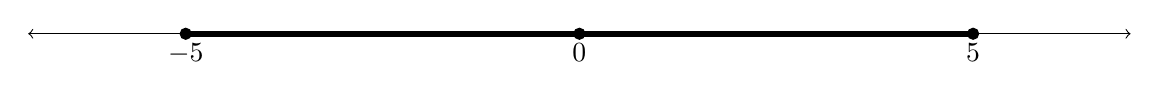
\begin{tikzpicture}
    % Draw the number line
    \draw[<->] (-7,0) -- (7,0);

    % Mark 0
    \draw[fill=black] (0,0) circle (2pt) node[below] {$0$};

    % Mark -5
    \draw[fill=black] (-5,0) circle (2pt) node[below] {$-5$};

    % Mark 5
    \draw[fill=black] (5,0) circle (2pt) node[below] {$5$};

    % Bold line between -5 and 5
    \draw[line width=2pt] (-5,0) -- (5,0);
\end{tikzpicture}
We can express this inequality without using absolute value. We know that $|x|<$5 is equivalent to $-5<x<5$. Because $x$ is somewhere between -5 and 5. Therefore the solution is $-5<x<5$. Or as an interval notation: $(-5,5)$.
\\
\vspace{4pt}
\textbf{Example.} What x-values satisfy $|x|\geq5$? \\
Since $|x|$ has to be greater than or equal to 5, $|x|$ has to be bigger then 5 and -5, since it can be both positive and negative. So, the x-values that satisfy the inequality are somewhere less than -5 or greater than 5. \\
\\
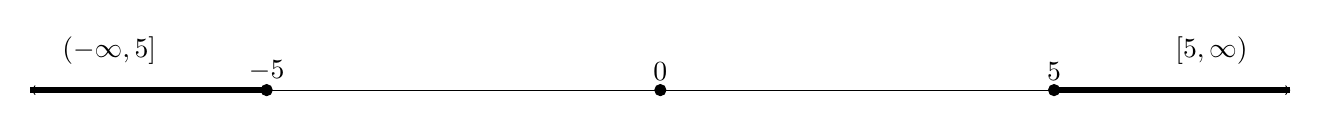
\begin{tikzpicture}
    % Draw the number line
    \draw[<->] (-8,0) -- (8,0);

    % Mark 0, 5, and -5 with filled circles
    \draw[fill=black] (0,0) circle (2pt) node[above] {$0$};
    \draw[fill=black] (5,0) circle (2pt) node[above] {$5$};
    \draw[fill=black] (-5,0) circle (2pt) node[above] {$-5$};

    % Mark the regions to be emphasized with bold lines
    \draw[line width=2pt] (-8,0) -- (-5,0);
    \draw[line width=2pt] (5,0) -- (8,0);

    % Label the emphasized regions
    \node at (-7,0.5) {$(-\infty, 5]$};
    \node at (7,0.5) {$[5, \infty)$};
\end{tikzpicture}

So, $x\leq-5$ or $x\geq5$. Or as an interval notation: $(-\infty, -5]\cup[5, \infty)$.

\textbf{Example.} Solve $|3-2t|<4$. 

Since $|3-2t|$ has to be less than 4 OR bigger -4 we can represent it in a numberline.  \\
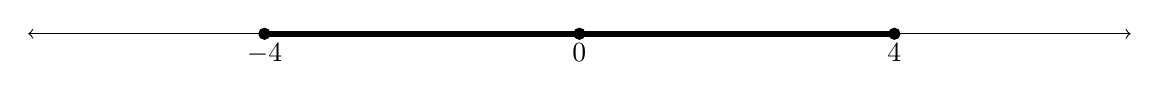
\begin{tikzpicture}
    % Draw the number line
    \draw[<->] (-7,0) -- (7,0);

    % Mark 0
    \draw[fill=black] (0,0) circle (2pt) node[below] {$0$};

    % Mark -5
    \draw[fill=black] (-4,0) circle (2pt) node[below] {$-4$};

    % Mark 5
    \draw[fill=black] (4,0) circle (2pt) node[below] {$4$};

    % Bold line between -5 and 5
    \draw[line width=2pt] (-4,0) -- (4,0);
\end{tikzpicture}

Therefore, we can just have two different equations: 
\begin{align*}
    3-2t<4 \\
    3-2t>-4
\end{align*}
Solving the first equation:
\begin{align*}
    3-2t<4 \\
    -2t<1 \\
    t>-\frac{1}{2}
\end{align*}
Solving the second equation:
\begin{align*}
    3-2t>-4 \\
    -2t>-7 \\
    t<\frac{7}{2}
\end{align*}

In the numberline we can see that the solution is $-\frac{1}{2}<t<\frac{7}{2}$. \\
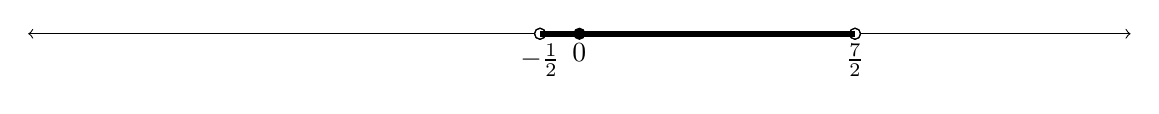
\begin{tikzpicture}
    % Draw the number line
    \draw[<->] (-7,0) -- (7,0);

    % Mark 0
    \draw[fill=black] (0,0) circle (2pt) node[below] {$0$};

    % Mark -1/2 with a hole
    \draw[fill=white] (-1/2,0) circle (2pt) node[below] {$-\frac{1}{2}$};
    \draw (-1/2,0) circle (2pt); % Draw a hole in the circle

    % Mark 7/2 with a hole
    \draw[fill=white] (7/2,0) circle (2pt) node[below] {$\frac{7}{2}$};
    \draw (7/2,0) circle (2pt); % Draw a hole in the circle

    % Bold line between -1/2 and 7/2
    \draw[line width=2pt] (-1/2,0) -- (7/2,0);
\end{tikzpicture}

Or as an interval notation: $(-\frac{1}{2}, \frac{7}{2})$.

Notice that the solution cannot include $-\frac{1}{2}$ and $\frac{7}{2}$ because $|3-2t|$ cannot be equal to 4. % Section 11 - Absolute Value Inequalities
\section{Algebraic Expressions}
A \textbf{variable} is a letter that can represent any number from a given set of numbers. If we
start with variables, such as $x$, $y$, and $z$, and some real numbers and combine them using
addition, subtraction, multiplication, division, powers, and roots, we obtain an \textbf{algebraic expression}. Here are some examples:

$$ 
    2x^2-3x+4 \quad \sqrt{x}+10 \quad \frac{y-2z}{y^2+4}
$$

A \textbf{monomial} is an expression of the form $ax^k$
, where a is a real number and k is a
nonnegative integer. A \textbf{binomial} is a sum of two monomials and a \textbf{trinomial} is a sum
of three monomials. In general, a sum of monomials is called a \textbf{polynomial}. For example, the first expression listed above is a polynomial, but the other two are not.

\begin{align*}
    \includegraphics[width=1.1\textwidth]{algebra-pre-calculus/algebra/algebraic-expressions/polynomial definition.png}
\end{align*} \break

Note that the degree of a polynomial is the highest power of the variable that appears
in the polynomial.


\begin{align*}
    \includegraphics[width=1.1\textwidth]{algebra-pre-calculus/algebra/algebraic-expressions/algebraic-expression-spreadsheet.png}
\end{align*} \break

We add and subtract polynomials using the properties of real numbers that were discussed earlier. The idea is to combine like terms (that is, terms with the same
variables raised to the same powers) using the Distributive Property. For instance,

$$ 
    5x^7+3x^7-2x^7 = (5+3-2)x^7 = 6x^7
$$

But we already know this. 

To find the product of polynomials or other algebraic expressions, we need to use the
Distributive Property repeatedly. In particular, using it three times on the product of two
binomials, we get

$$ 
    (a+b)(c+d) = a(c+d)+b(c+d) = ac+ad+bc+bd
$$

\subsection{Special Product Formulas}
Certain types of products occur so frequently that you should memorize them. You can
verify the following formulas by performing the multiplications.

\begin{align*}
    \includegraphics[width=1.1\textwidth]{algebra-pre-calculus/algebra/algebraic-expressions/special_product_formulas.png}
\end{align*} \break

\subsection{Factoring Common Factors}
We use the Distributive Property to expand algebraic expressions. We sometimes need
to reverse this process (again using the Distributive Property) by factoring an expression as a product of simpler ones.
For example,
\begin{align*}
    &A. \quad 15 + 25x = 5(3 + 5x) \\
    &B. \quad x^2y + y^2x^3 = x^2y(1 + xy) \\
\end{align*}
You can always check whether you have factored correctly by expanding the brackets.

\subsection{Factoring quadratics}
A quadratic is an expression with a squared term, then just a term with a variable, then a constant. 
\\ Like this: $ax^2 + bx + c$ 
More about solving quadratic equations and quadratic equations in general can be found in the next section \hyperref[sec:quadratic-equations]{Quadratic Equations(click to redirect)}.


We are looking for two numbers that multiply you get $c$ and when you add them you get $b$.
The reason why: 
$$ (x + m)(x + n) = \\ x^2 + mx + nx + mn = x^2 + \underbrace{(m + n)}_b x + \underbrace{(mn)}_c $$

$m$ and $n$ are the two numbers we are looking for. As you can see $m + n = b$ and $mn = c$. \\

\textbf{Example}. Factor $x^2 - 6x + 8$ \\
We are looking for two numbers that multiply you get $8$ and when you add them you get $-6$. \\
The two numbers are $-2$ and $-4$ because $-2 \cdot -4 = 8$ and $-2 + -4 = -6$. \\
Therefore, 
\begin{align*}
    x^2 - 6x + 8 &= (x - 2)(x - 4) \\
\end{align*}

\textbf{Example}. Factor $10x^2 + 11x - 6$ \\
\begin{itemize}
    \item Step 1. Multiply the leading coefficient (10) and the constant term (-6) to get -60. \\
    \textbf{Why?} The main goal in factoring a quadratic equation is to express it as the product of two binomials(like (2x+4)(4x+5)). 
    In the case of a quadratic with a leading coefficient (the coefficient of $x^2$) not equal to 1, like $10x^2$ in our example, we need to find two binomials of the form $(ax + b)(cx + d)$ e.g $(2x + 4)(5x+2)$ such that their product equals the given quadratic. 
    So, in this context, we are essentially trying to break down the original quadratic ($10x^2 - 11x - 6$) into two binomials, and we start by looking for two numbers that will help us achieve this. These two numbers should meet two criteria:
    \begin{itemize}
        \item Their product should equal the product of the leading coefficient and the constant term (in this case, $10 \cdot -6 = -60$).
        \item Their sum should equal the coefficient of the x-term (in this case, -11)
    \end{itemize}
    By finding such numbers, we can rewrite the middle term of the quadratic equation (the -11x term) as the sum or difference of two terms, each of which can be factored more easily. This allows us to perform factoring by grouping, making the overall factoring process more manageable.
    \item Step 2.  Find two numbers that multiply to -60 and add up to the coefficient of the x-term (-11). In this case, those two numbers are -15 and 4 because $(-15) \cdot 4 = -60$ and $(-15) + 4 = -11$.
    \item Step 3. Rewrite the middle term (-11x) using the two numbers found in step 2: 
    $$ 10x^2 - 15x + 4x - 6 $$
    \item Step 4. Group the terms: Group the first two terms $(10x^2 - 15x)$ and the last two terms $(4x - 6)$. This will gve us: 
    $$ 5x(2x - 3) + 2(2x - 3) $$
    \item Step 5. Factor out the HCF of each group: 
    $$ 5x(2x - 3) + 2(2x - 3) = (5x + 2)(2x - 3) $$

\end{itemize}
And we are done factorising the quadratic equation.

\subsection{Difference of squares}
The difference of squares is a squared term minus another squared term.
\\ Like this: $a^2 - b^2 = (a+b)(a-b) = a^2-ab+ab-b^2 $ 

\textbf{Example.} Factor $x^2 - 9$ 
$$ (x+3)(x-3) $$


\textbf{Example.} Factor $9p^2 - 1$ 
$$ (3p+1)(3p-1) $$

\subsection{Difference or sum of cubes}
The difference or sum of cubes is a cubed term plus or minus another cubed term.

$$ a^3 - b^3 = (a-b)(a^2+ab+b^2) $$ Because, $$(a-b)(a^2+ab+b^2) = a^3 - ab^2 + a^2b - ab^2 + b^3 = a^3 - 2ab^2 + b^3 $$ 

And, 
$$ a^3 + b^3 = (a+b)(a^2-ab+b^2) $$ Because, $$(a+b)(a^2-ab+b^2) = a^3 + ab^2 - a^2b + ab^2 + b^3 = a^3 + 2ab^2 + b^3 $$ 
\\
\textbf{Example.} Factor $x^3 - 8$ \\
We know that $x^3 - 8 = x^3 - 2^3$
Therefore,
$$ (x-2)(x^2+2x+4) $$

if we expand out: 
$$ (x-2)(x^2+2x+4) = x^3 + 2x^2 + 4x - 2x^2 - 4x - 8 = x^3 - 8 $$
Therefore our answer is correct.

\subsection{Additional examples of factoring}
\textbf{Example.} Which of these expressions DOES NOT factorise?

A. $x^2 + x$ \\
This can be factored by pulling out the highest common factor. \\
$$ x^2 + x = x(x+1) $$

B. $x^2 - 25$ \\
This also can be factored by difference of squares. \\
$$ x^2 - 25 = (x+5)(x-5) $$

C. $x^2 + 4$ \\
This cannot be factored because it is a sum of squares not a difference of squares. \\

D. $x^3+2x^2+3x+6$ \\
This can also be factored by grouping. \\
$$ x^3+2x^2+3x+6 = x^2(x+2)+3(x+2) = (x^2+3)(x+2) $$

E. $5x^2-14x+8$ \\
This can also be factored by using the method of factoring quadratics when $a \neq 1$. \\
Therefore we can multiply the leading coefficient (5) and the constant term (8) to get 40. \\
We are looking for two numbers that multiply you get 40 and when you add them you get -14 and those are -10 and -4. \\
So we can rewrite the middle term (-14x) using the two numbers found:
$$ 5x^2 - 10x - 4x + 8 $$ 
Then we can group them together:
$$ 5x(x - 2) - 4(x - 2) $$
And finally factor out the HCF of each group:
$$ (5x - 4)(x - 2) $$

Eventually the answer for our question is C. $x^2 + 4$ because it cannot be factored.

\subsection{Tips and Extra examples}
\begin{itemize}
    \item Always look for the highest common factor first. That will simplify things and make the rest of the factoring more easier. 
    \item You might need to do several steps of factoring to get the final answer. For example you might have to pull out the HCF first then you can do factoring by grouping or factoring quadratics. Then you might also apply difference of squares or difference or sum of cubes. Keep factoring as far as you can go.
\end{itemize}

\textbf{Extra Example} Factor $2z^2 + 3z -14$ \\
Again as previously done first we need to multiply the leading coefficient (2) and the constant term (-14) to get -28. \\ 
We are looking for two numbers that multiply you get -28 and when you add them you get 3 and those are 7 and -4. \\
So we can rewrite the middle term (3z) using the two numbers found:
$$ 2z^2 + 7z - 4z - 14 $$ 
Then we can group them together:
$$ z(2z + 7) - 2(2z + 7) $$
And finally factor out the HCF of each group:
$$ (z - 2)(2z + 7) $$

\textbf{Extra Example} Factor $-5v^2-45v+50$ \\
Again as previously done first we need to multiply the leading coefficient (-5) and the constant term (50) to get -250. \\
We are looking for two numbers that multiply you get -250 and when you add them you get -45 and those are -50 and 5. \\
So we can rewrite the middle term (-45v) using the two numbers found:
$$ -5v^2 - 50v + 5v + 50 $$ 
Then we can group them together:
$$ -5v(v + 10) + 5(v + 10) $$
And finally factor out the HCF of each group:
$$ (-5v + 5)(v + 10) $$
This can be further simplified to:
$$ -5(v - 1)(v + 10) $$
Another solution for this could have been that first we could have pulled out the HCF which is -5 and then we could have factored the quadratic. \\
$$ -5v^2 - 45v + 50 = -5(v^2 + 9v - 10) $$
And this is really easy since $ a = 1 $ Therefore we need two numbers that multiply you get -10 and when you add them you get 9 and those are 10 and -1. \\
So we can say that: 
$$ -5(v^2 + 9v - 10) = -5(v + 10)(v - 1) $$

\subsection{Special Factoring Formulas}
\begin{align*}
    \includegraphics[width=1.1\textwidth]{algebra-pre-calculus/algebra/algebraic-expressions/special_factoring_formulas.png}
\end{align*} \break

When we factor an expression, the result can sometimes be factored further. In general, we first factor out common factors, then inspect the result to see whether it can be
factored by any of the other methods of this section. We repeat this process until we
have factored the expression completely

\subsection{Factoring Expressions with Fractional Exponents}
Factor each expresson. \\ \break
\textbf{(a)} \scalebox{1.2}{$3x^{\frac{3}{2}}-9x^{\frac{1}{2}}+6x^{-\frac{1}{2}}$ = $3x^{-\frac{1}{2}}(x^2-3x+2)$ = $3x^{-\frac{1}{2}}(x-2)(x-1)$} \\ \break
Here we have taken the common factor $3x^{-\frac{1}{2}}$ out of each term. Then we have factored the quadratic expression $x^2-3x+2$. \\ \break

\textbf{(b)} $(2+x)^{-\frac{2}{3}}x+(2+x)^{\frac{1}{3}} = (2+x)^{-\frac{2}{3}}[x+(2+x)] = (2+x)^{-\frac{2}{3}}(x+2+x) = (2+x)^{-\frac{2}{3}}(2x+2)$ \\ \break
Here we have taken the common factor $(2+x)^{-\frac{2}{3}}$ out of each term. Then we have just simplified. \\ \break % Section 12 - Solving Absolute Value Equations
\section{Algebraic Expressions}
A \textbf{variable} is a letter that can represent any number from a given set of numbers. If we
start with variables, such as $x$, $y$, and $z$, and some real numbers and combine them using
addition, subtraction, multiplication, division, powers, and roots, we obtain an \textbf{algebraic expression}. Here are some examples:

$$ 
    2x^2-3x+4 \quad \sqrt{x}+10 \quad \frac{y-2z}{y^2+4}
$$

A \textbf{monomial} is an expression of the form $ax^k$
, where a is a real number and k is a
nonnegative integer. A \textbf{binomial} is a sum of two monomials and a \textbf{trinomial} is a sum
of three monomials. In general, a sum of monomials is called a \textbf{polynomial}. For example, the first expression listed above is a polynomial, but the other two are not.

\begin{align*}
    \includegraphics[width=1.1\textwidth]{algebra-pre-calculus/algebra/algebraic-expressions/polynomial definition.png}
\end{align*} \break

Note that the degree of a polynomial is the highest power of the variable that appears
in the polynomial.


\begin{align*}
    \includegraphics[width=1.1\textwidth]{algebra-pre-calculus/algebra/algebraic-expressions/algebraic-expression-spreadsheet.png}
\end{align*} \break

We add and subtract polynomials using the properties of real numbers that were discussed earlier. The idea is to combine like terms (that is, terms with the same
variables raised to the same powers) using the Distributive Property. For instance,

$$ 
    5x^7+3x^7-2x^7 = (5+3-2)x^7 = 6x^7
$$

But we already know this. 

To find the product of polynomials or other algebraic expressions, we need to use the
Distributive Property repeatedly. In particular, using it three times on the product of two
binomials, we get

$$ 
    (a+b)(c+d) = a(c+d)+b(c+d) = ac+ad+bc+bd
$$

\subsection{Special Product Formulas}
Certain types of products occur so frequently that you should memorize them. You can
verify the following formulas by performing the multiplications.

\begin{align*}
    \includegraphics[width=1.1\textwidth]{algebra-pre-calculus/algebra/algebraic-expressions/special_product_formulas.png}
\end{align*} \break

\subsection{Factoring Common Factors}
We use the Distributive Property to expand algebraic expressions. We sometimes need
to reverse this process (again using the Distributive Property) by factoring an expression as a product of simpler ones.
For example,
\begin{align*}
    &A. \quad 15 + 25x = 5(3 + 5x) \\
    &B. \quad x^2y + y^2x^3 = x^2y(1 + xy) \\
\end{align*}
You can always check whether you have factored correctly by expanding the brackets.

\subsection{Factoring quadratics}
A quadratic is an expression with a squared term, then just a term with a variable, then a constant. 
\\ Like this: $ax^2 + bx + c$ 
More about solving quadratic equations and quadratic equations in general can be found in the next section \hyperref[sec:quadratic-equations]{Quadratic Equations(click to redirect)}.


We are looking for two numbers that multiply you get $c$ and when you add them you get $b$.
The reason why: 
$$ (x + m)(x + n) = \\ x^2 + mx + nx + mn = x^2 + \underbrace{(m + n)}_b x + \underbrace{(mn)}_c $$

$m$ and $n$ are the two numbers we are looking for. As you can see $m + n = b$ and $mn = c$. \\

\textbf{Example}. Factor $x^2 - 6x + 8$ \\
We are looking for two numbers that multiply you get $8$ and when you add them you get $-6$. \\
The two numbers are $-2$ and $-4$ because $-2 \cdot -4 = 8$ and $-2 + -4 = -6$. \\
Therefore, 
\begin{align*}
    x^2 - 6x + 8 &= (x - 2)(x - 4) \\
\end{align*}

\textbf{Example}. Factor $10x^2 + 11x - 6$ \\
\begin{itemize}
    \item Step 1. Multiply the leading coefficient (10) and the constant term (-6) to get -60. \\
    \textbf{Why?} The main goal in factoring a quadratic equation is to express it as the product of two binomials(like (2x+4)(4x+5)). 
    In the case of a quadratic with a leading coefficient (the coefficient of $x^2$) not equal to 1, like $10x^2$ in our example, we need to find two binomials of the form $(ax + b)(cx + d)$ e.g $(2x + 4)(5x+2)$ such that their product equals the given quadratic. 
    So, in this context, we are essentially trying to break down the original quadratic ($10x^2 - 11x - 6$) into two binomials, and we start by looking for two numbers that will help us achieve this. These two numbers should meet two criteria:
    \begin{itemize}
        \item Their product should equal the product of the leading coefficient and the constant term (in this case, $10 \cdot -6 = -60$).
        \item Their sum should equal the coefficient of the x-term (in this case, -11)
    \end{itemize}
    By finding such numbers, we can rewrite the middle term of the quadratic equation (the -11x term) as the sum or difference of two terms, each of which can be factored more easily. This allows us to perform factoring by grouping, making the overall factoring process more manageable.
    \item Step 2.  Find two numbers that multiply to -60 and add up to the coefficient of the x-term (-11). In this case, those two numbers are -15 and 4 because $(-15) \cdot 4 = -60$ and $(-15) + 4 = -11$.
    \item Step 3. Rewrite the middle term (-11x) using the two numbers found in step 2: 
    $$ 10x^2 - 15x + 4x - 6 $$
    \item Step 4. Group the terms: Group the first two terms $(10x^2 - 15x)$ and the last two terms $(4x - 6)$. This will gve us: 
    $$ 5x(2x - 3) + 2(2x - 3) $$
    \item Step 5. Factor out the HCF of each group: 
    $$ 5x(2x - 3) + 2(2x - 3) = (5x + 2)(2x - 3) $$

\end{itemize}
And we are done factorising the quadratic equation.

\subsection{Difference of squares}
The difference of squares is a squared term minus another squared term.
\\ Like this: $a^2 - b^2 = (a+b)(a-b) = a^2-ab+ab-b^2 $ 

\textbf{Example.} Factor $x^2 - 9$ 
$$ (x+3)(x-3) $$


\textbf{Example.} Factor $9p^2 - 1$ 
$$ (3p+1)(3p-1) $$

\subsection{Difference or sum of cubes}
The difference or sum of cubes is a cubed term plus or minus another cubed term.

$$ a^3 - b^3 = (a-b)(a^2+ab+b^2) $$ Because, $$(a-b)(a^2+ab+b^2) = a^3 - ab^2 + a^2b - ab^2 + b^3 = a^3 - 2ab^2 + b^3 $$ 

And, 
$$ a^3 + b^3 = (a+b)(a^2-ab+b^2) $$ Because, $$(a+b)(a^2-ab+b^2) = a^3 + ab^2 - a^2b + ab^2 + b^3 = a^3 + 2ab^2 + b^3 $$ 
\\
\textbf{Example.} Factor $x^3 - 8$ \\
We know that $x^3 - 8 = x^3 - 2^3$
Therefore,
$$ (x-2)(x^2+2x+4) $$

if we expand out: 
$$ (x-2)(x^2+2x+4) = x^3 + 2x^2 + 4x - 2x^2 - 4x - 8 = x^3 - 8 $$
Therefore our answer is correct.

\subsection{Additional examples of factoring}
\textbf{Example.} Which of these expressions DOES NOT factorise?

A. $x^2 + x$ \\
This can be factored by pulling out the highest common factor. \\
$$ x^2 + x = x(x+1) $$

B. $x^2 - 25$ \\
This also can be factored by difference of squares. \\
$$ x^2 - 25 = (x+5)(x-5) $$

C. $x^2 + 4$ \\
This cannot be factored because it is a sum of squares not a difference of squares. \\

D. $x^3+2x^2+3x+6$ \\
This can also be factored by grouping. \\
$$ x^3+2x^2+3x+6 = x^2(x+2)+3(x+2) = (x^2+3)(x+2) $$

E. $5x^2-14x+8$ \\
This can also be factored by using the method of factoring quadratics when $a \neq 1$. \\
Therefore we can multiply the leading coefficient (5) and the constant term (8) to get 40. \\
We are looking for two numbers that multiply you get 40 and when you add them you get -14 and those are -10 and -4. \\
So we can rewrite the middle term (-14x) using the two numbers found:
$$ 5x^2 - 10x - 4x + 8 $$ 
Then we can group them together:
$$ 5x(x - 2) - 4(x - 2) $$
And finally factor out the HCF of each group:
$$ (5x - 4)(x - 2) $$

Eventually the answer for our question is C. $x^2 + 4$ because it cannot be factored.

\subsection{Tips and Extra examples}
\begin{itemize}
    \item Always look for the highest common factor first. That will simplify things and make the rest of the factoring more easier. 
    \item You might need to do several steps of factoring to get the final answer. For example you might have to pull out the HCF first then you can do factoring by grouping or factoring quadratics. Then you might also apply difference of squares or difference or sum of cubes. Keep factoring as far as you can go.
\end{itemize}

\textbf{Extra Example} Factor $2z^2 + 3z -14$ \\
Again as previously done first we need to multiply the leading coefficient (2) and the constant term (-14) to get -28. \\ 
We are looking for two numbers that multiply you get -28 and when you add them you get 3 and those are 7 and -4. \\
So we can rewrite the middle term (3z) using the two numbers found:
$$ 2z^2 + 7z - 4z - 14 $$ 
Then we can group them together:
$$ z(2z + 7) - 2(2z + 7) $$
And finally factor out the HCF of each group:
$$ (z - 2)(2z + 7) $$

\textbf{Extra Example} Factor $-5v^2-45v+50$ \\
Again as previously done first we need to multiply the leading coefficient (-5) and the constant term (50) to get -250. \\
We are looking for two numbers that multiply you get -250 and when you add them you get -45 and those are -50 and 5. \\
So we can rewrite the middle term (-45v) using the two numbers found:
$$ -5v^2 - 50v + 5v + 50 $$ 
Then we can group them together:
$$ -5v(v + 10) + 5(v + 10) $$
And finally factor out the HCF of each group:
$$ (-5v + 5)(v + 10) $$
This can be further simplified to:
$$ -5(v - 1)(v + 10) $$
Another solution for this could have been that first we could have pulled out the HCF which is -5 and then we could have factored the quadratic. \\
$$ -5v^2 - 45v + 50 = -5(v^2 + 9v - 10) $$
And this is really easy since $ a = 1 $ Therefore we need two numbers that multiply you get -10 and when you add them you get 9 and those are 10 and -1. \\
So we can say that: 
$$ -5(v^2 + 9v - 10) = -5(v + 10)(v - 1) $$

\subsection{Special Factoring Formulas}
\begin{align*}
    \includegraphics[width=1.1\textwidth]{algebra-pre-calculus/algebra/algebraic-expressions/special_factoring_formulas.png}
\end{align*} \break

When we factor an expression, the result can sometimes be factored further. In general, we first factor out common factors, then inspect the result to see whether it can be
factored by any of the other methods of this section. We repeat this process until we
have factored the expression completely

\subsection{Factoring Expressions with Fractional Exponents}
Factor each expresson. \\ \break
\textbf{(a)} \scalebox{1.2}{$3x^{\frac{3}{2}}-9x^{\frac{1}{2}}+6x^{-\frac{1}{2}}$ = $3x^{-\frac{1}{2}}(x^2-3x+2)$ = $3x^{-\frac{1}{2}}(x-2)(x-1)$} \\ \break
Here we have taken the common factor $3x^{-\frac{1}{2}}$ out of each term. Then we have factored the quadratic expression $x^2-3x+2$. \\ \break

\textbf{(b)} $(2+x)^{-\frac{2}{3}}x+(2+x)^{\frac{1}{3}} = (2+x)^{-\frac{2}{3}}[x+(2+x)] = (2+x)^{-\frac{2}{3}}(x+2+x) = (2+x)^{-\frac{2}{3}}(2x+2)$ \\ \break
Here we have taken the common factor $(2+x)^{-\frac{2}{3}}$ out of each term. Then we have just simplified. \\ \break % Section 13 - Solving Rational Equations
\section{Algebraic Expressions}
A \textbf{variable} is a letter that can represent any number from a given set of numbers. If we
start with variables, such as $x$, $y$, and $z$, and some real numbers and combine them using
addition, subtraction, multiplication, division, powers, and roots, we obtain an \textbf{algebraic expression}. Here are some examples:

$$ 
    2x^2-3x+4 \quad \sqrt{x}+10 \quad \frac{y-2z}{y^2+4}
$$

A \textbf{monomial} is an expression of the form $ax^k$
, where a is a real number and k is a
nonnegative integer. A \textbf{binomial} is a sum of two monomials and a \textbf{trinomial} is a sum
of three monomials. In general, a sum of monomials is called a \textbf{polynomial}. For example, the first expression listed above is a polynomial, but the other two are not.

\begin{align*}
    \includegraphics[width=1.1\textwidth]{algebra-pre-calculus/algebra/algebraic-expressions/polynomial definition.png}
\end{align*} \break

Note that the degree of a polynomial is the highest power of the variable that appears
in the polynomial.


\begin{align*}
    \includegraphics[width=1.1\textwidth]{algebra-pre-calculus/algebra/algebraic-expressions/algebraic-expression-spreadsheet.png}
\end{align*} \break

We add and subtract polynomials using the properties of real numbers that were discussed earlier. The idea is to combine like terms (that is, terms with the same
variables raised to the same powers) using the Distributive Property. For instance,

$$ 
    5x^7+3x^7-2x^7 = (5+3-2)x^7 = 6x^7
$$

But we already know this. 

To find the product of polynomials or other algebraic expressions, we need to use the
Distributive Property repeatedly. In particular, using it three times on the product of two
binomials, we get

$$ 
    (a+b)(c+d) = a(c+d)+b(c+d) = ac+ad+bc+bd
$$

\subsection{Special Product Formulas}
Certain types of products occur so frequently that you should memorize them. You can
verify the following formulas by performing the multiplications.

\begin{align*}
    \includegraphics[width=1.1\textwidth]{algebra-pre-calculus/algebra/algebraic-expressions/special_product_formulas.png}
\end{align*} \break

\subsection{Factoring Common Factors}
We use the Distributive Property to expand algebraic expressions. We sometimes need
to reverse this process (again using the Distributive Property) by factoring an expression as a product of simpler ones.
For example,
\begin{align*}
    &A. \quad 15 + 25x = 5(3 + 5x) \\
    &B. \quad x^2y + y^2x^3 = x^2y(1 + xy) \\
\end{align*}
You can always check whether you have factored correctly by expanding the brackets.

\subsection{Factoring quadratics}
A quadratic is an expression with a squared term, then just a term with a variable, then a constant. 
\\ Like this: $ax^2 + bx + c$ 
More about solving quadratic equations and quadratic equations in general can be found in the next section \hyperref[sec:quadratic-equations]{Quadratic Equations(click to redirect)}.


We are looking for two numbers that multiply you get $c$ and when you add them you get $b$.
The reason why: 
$$ (x + m)(x + n) = \\ x^2 + mx + nx + mn = x^2 + \underbrace{(m + n)}_b x + \underbrace{(mn)}_c $$

$m$ and $n$ are the two numbers we are looking for. As you can see $m + n = b$ and $mn = c$. \\

\textbf{Example}. Factor $x^2 - 6x + 8$ \\
We are looking for two numbers that multiply you get $8$ and when you add them you get $-6$. \\
The two numbers are $-2$ and $-4$ because $-2 \cdot -4 = 8$ and $-2 + -4 = -6$. \\
Therefore, 
\begin{align*}
    x^2 - 6x + 8 &= (x - 2)(x - 4) \\
\end{align*}

\textbf{Example}. Factor $10x^2 + 11x - 6$ \\
\begin{itemize}
    \item Step 1. Multiply the leading coefficient (10) and the constant term (-6) to get -60. \\
    \textbf{Why?} The main goal in factoring a quadratic equation is to express it as the product of two binomials(like (2x+4)(4x+5)). 
    In the case of a quadratic with a leading coefficient (the coefficient of $x^2$) not equal to 1, like $10x^2$ in our example, we need to find two binomials of the form $(ax + b)(cx + d)$ e.g $(2x + 4)(5x+2)$ such that their product equals the given quadratic. 
    So, in this context, we are essentially trying to break down the original quadratic ($10x^2 - 11x - 6$) into two binomials, and we start by looking for two numbers that will help us achieve this. These two numbers should meet two criteria:
    \begin{itemize}
        \item Their product should equal the product of the leading coefficient and the constant term (in this case, $10 \cdot -6 = -60$).
        \item Their sum should equal the coefficient of the x-term (in this case, -11)
    \end{itemize}
    By finding such numbers, we can rewrite the middle term of the quadratic equation (the -11x term) as the sum or difference of two terms, each of which can be factored more easily. This allows us to perform factoring by grouping, making the overall factoring process more manageable.
    \item Step 2.  Find two numbers that multiply to -60 and add up to the coefficient of the x-term (-11). In this case, those two numbers are -15 and 4 because $(-15) \cdot 4 = -60$ and $(-15) + 4 = -11$.
    \item Step 3. Rewrite the middle term (-11x) using the two numbers found in step 2: 
    $$ 10x^2 - 15x + 4x - 6 $$
    \item Step 4. Group the terms: Group the first two terms $(10x^2 - 15x)$ and the last two terms $(4x - 6)$. This will gve us: 
    $$ 5x(2x - 3) + 2(2x - 3) $$
    \item Step 5. Factor out the HCF of each group: 
    $$ 5x(2x - 3) + 2(2x - 3) = (5x + 2)(2x - 3) $$

\end{itemize}
And we are done factorising the quadratic equation.

\subsection{Difference of squares}
The difference of squares is a squared term minus another squared term.
\\ Like this: $a^2 - b^2 = (a+b)(a-b) = a^2-ab+ab-b^2 $ 

\textbf{Example.} Factor $x^2 - 9$ 
$$ (x+3)(x-3) $$


\textbf{Example.} Factor $9p^2 - 1$ 
$$ (3p+1)(3p-1) $$

\subsection{Difference or sum of cubes}
The difference or sum of cubes is a cubed term plus or minus another cubed term.

$$ a^3 - b^3 = (a-b)(a^2+ab+b^2) $$ Because, $$(a-b)(a^2+ab+b^2) = a^3 - ab^2 + a^2b - ab^2 + b^3 = a^3 - 2ab^2 + b^3 $$ 

And, 
$$ a^3 + b^3 = (a+b)(a^2-ab+b^2) $$ Because, $$(a+b)(a^2-ab+b^2) = a^3 + ab^2 - a^2b + ab^2 + b^3 = a^3 + 2ab^2 + b^3 $$ 
\\
\textbf{Example.} Factor $x^3 - 8$ \\
We know that $x^3 - 8 = x^3 - 2^3$
Therefore,
$$ (x-2)(x^2+2x+4) $$

if we expand out: 
$$ (x-2)(x^2+2x+4) = x^3 + 2x^2 + 4x - 2x^2 - 4x - 8 = x^3 - 8 $$
Therefore our answer is correct.

\subsection{Additional examples of factoring}
\textbf{Example.} Which of these expressions DOES NOT factorise?

A. $x^2 + x$ \\
This can be factored by pulling out the highest common factor. \\
$$ x^2 + x = x(x+1) $$

B. $x^2 - 25$ \\
This also can be factored by difference of squares. \\
$$ x^2 - 25 = (x+5)(x-5) $$

C. $x^2 + 4$ \\
This cannot be factored because it is a sum of squares not a difference of squares. \\

D. $x^3+2x^2+3x+6$ \\
This can also be factored by grouping. \\
$$ x^3+2x^2+3x+6 = x^2(x+2)+3(x+2) = (x^2+3)(x+2) $$

E. $5x^2-14x+8$ \\
This can also be factored by using the method of factoring quadratics when $a \neq 1$. \\
Therefore we can multiply the leading coefficient (5) and the constant term (8) to get 40. \\
We are looking for two numbers that multiply you get 40 and when you add them you get -14 and those are -10 and -4. \\
So we can rewrite the middle term (-14x) using the two numbers found:
$$ 5x^2 - 10x - 4x + 8 $$ 
Then we can group them together:
$$ 5x(x - 2) - 4(x - 2) $$
And finally factor out the HCF of each group:
$$ (5x - 4)(x - 2) $$

Eventually the answer for our question is C. $x^2 + 4$ because it cannot be factored.

\subsection{Tips and Extra examples}
\begin{itemize}
    \item Always look for the highest common factor first. That will simplify things and make the rest of the factoring more easier. 
    \item You might need to do several steps of factoring to get the final answer. For example you might have to pull out the HCF first then you can do factoring by grouping or factoring quadratics. Then you might also apply difference of squares or difference or sum of cubes. Keep factoring as far as you can go.
\end{itemize}

\textbf{Extra Example} Factor $2z^2 + 3z -14$ \\
Again as previously done first we need to multiply the leading coefficient (2) and the constant term (-14) to get -28. \\ 
We are looking for two numbers that multiply you get -28 and when you add them you get 3 and those are 7 and -4. \\
So we can rewrite the middle term (3z) using the two numbers found:
$$ 2z^2 + 7z - 4z - 14 $$ 
Then we can group them together:
$$ z(2z + 7) - 2(2z + 7) $$
And finally factor out the HCF of each group:
$$ (z - 2)(2z + 7) $$

\textbf{Extra Example} Factor $-5v^2-45v+50$ \\
Again as previously done first we need to multiply the leading coefficient (-5) and the constant term (50) to get -250. \\
We are looking for two numbers that multiply you get -250 and when you add them you get -45 and those are -50 and 5. \\
So we can rewrite the middle term (-45v) using the two numbers found:
$$ -5v^2 - 50v + 5v + 50 $$ 
Then we can group them together:
$$ -5v(v + 10) + 5(v + 10) $$
And finally factor out the HCF of each group:
$$ (-5v + 5)(v + 10) $$
This can be further simplified to:
$$ -5(v - 1)(v + 10) $$
Another solution for this could have been that first we could have pulled out the HCF which is -5 and then we could have factored the quadratic. \\
$$ -5v^2 - 45v + 50 = -5(v^2 + 9v - 10) $$
And this is really easy since $ a = 1 $ Therefore we need two numbers that multiply you get -10 and when you add them you get 9 and those are 10 and -1. \\
So we can say that: 
$$ -5(v^2 + 9v - 10) = -5(v + 10)(v - 1) $$

\subsection{Special Factoring Formulas}
\begin{align*}
    \includegraphics[width=1.1\textwidth]{algebra-pre-calculus/algebra/algebraic-expressions/special_factoring_formulas.png}
\end{align*} \break

When we factor an expression, the result can sometimes be factored further. In general, we first factor out common factors, then inspect the result to see whether it can be
factored by any of the other methods of this section. We repeat this process until we
have factored the expression completely

\subsection{Factoring Expressions with Fractional Exponents}
Factor each expresson. \\ \break
\textbf{(a)} \scalebox{1.2}{$3x^{\frac{3}{2}}-9x^{\frac{1}{2}}+6x^{-\frac{1}{2}}$ = $3x^{-\frac{1}{2}}(x^2-3x+2)$ = $3x^{-\frac{1}{2}}(x-2)(x-1)$} \\ \break
Here we have taken the common factor $3x^{-\frac{1}{2}}$ out of each term. Then we have factored the quadratic expression $x^2-3x+2$. \\ \break

\textbf{(b)} $(2+x)^{-\frac{2}{3}}x+(2+x)^{\frac{1}{3}} = (2+x)^{-\frac{2}{3}}[x+(2+x)] = (2+x)^{-\frac{2}{3}}(x+2+x) = (2+x)^{-\frac{2}{3}}(2x+2)$ \\ \break
Here we have taken the common factor $(2+x)^{-\frac{2}{3}}$ out of each term. Then we have just simplified. \\ \break % Section 14 - Summations
\section{Complex numbers}

From the section \hyperref[sec:equations]{Equations} we saw that if the discriminant of a quadratic equation is negative, the
equation has no real solution. For example, the equation $$x^2+4=0$$ has no real solution. If we try to solve this equation, we get $x^2=-4$, so $$x=\pm \sqrt{-4}$$
But this is impossible, since the square of any real number is positive. [For example, $(-2)^2=4$, a positive number.] Thus negative numbers don’t have real square roots.
To make it possible to solve all quadratic equations, mathematicians invented an
expanded number system, called the complex number system. First they defined the new
number $i$ which is, $$i=\sqrt{-1}$$ This means that $i^2=-1$. A complex number is then a number of the form $a+bi$, where $a$ and $b$ are real numbers.

\begin{align*}
    \includegraphics[width=1.1\textwidth]{algebra-pre-calculus/algebra/complex-numbers/complex_numbers_def.png}
\end{align*}

In the complex number the reason why $b$ is being called as the \textbf{imaginary part} is not because it's an imaginary number(when squared produce negative outcome). It's because it's being multiplied by the imaginary number $i$, so it's kind of the "part" of it. The real part is the part that is \textbf{not} being multiplied by $i$. \\

Note that both the real and the imaginary part are real numbers.

A number such as $6i$, which has real part 0, is called a \textbf{pure imaginary number}. A
real number such as $-7$ can be thought of as a complex number with imaginary part 0.
In the complex number system every quadratic equation has solutions. The numbers
$2i$ and $-2i$ are solutions of $x^2-4$ because

\begin{align*}
    (2i)^2  & =4i^2=-4 \\
    (-2i)^2 & =4i^2=-4
\end{align*}

We study complex numbers because they complete, in a useful and elegant
fashion, our study of the solutions of equations. In fact, imaginary numbers are useful not
only in algebra and mathematics, but in the other sciences as well. To give just one example, in electrical theory the reactance of a circuit is a quantity whose measure is an
imaginary number. \\

\subsection{Arithmetic Operations on Complex Numbers}

Complex numbers are added, subtracted, multiplied, and divided just as we would any
number of the form $a+b\sqrt{c}$. The only difference that we need to keep in mind is that $i^2=-1$. Thus the following calculations are valid.

\begin{align*}
    (a+bi)(c+di) & = ac+adi+bci+bdi^2 \\
                 & =ac+(ad+bc)i-bd    \\
                 & = (ac-bd)+(ad+bc)i
\end{align*}

\begin{align*}
    \includegraphics[width=1.1\textwidth]{algebra-pre-calculus/algebra/complex-numbers/arithmetic_operations_complex_numbers.png}
\end{align*}

\subsection{Examples of Adding and subtracting complex numbers}
Express the following complex numbers in the form $a+bi$. \\
\textbf{(a)} $(3+5i)+(4-2i)=(3+4)+(5-2)i=7+3i$ \\
\textbf{(b)} $(3+5i)-(4-2)=(3-4)[5-(-2i)]i=-1+7i$ \\
\textbf{(c)} $(3+5i)(4-2i) = 12-6i+20i-10i^2=12+14i+10=22+14i$ \\
\textbf{(d)} $i^{23}=i^{22+1}=(i^2)^{11}i=(-1)^{11}i=-i$ \\

\subsection{Dividing Complex Numbers}
Division of complex numbers is much like rationalizing the denominator of a radical expression. For the complex number $z=a+bi$ we define its \textbf{complex conjugate} to be the complex number $\overline{z}=a-bi$. The complex conjugate of $z$ is obtained by changing the sign of the imaginary part of $z$. For example, the complex conjugate of $3+5i$ is $3-5i$. \\
Note that, $$z\cdot\overline{z}=(a+bi)(a-bi)=a^2-(bi)^2=a^2+b^2$$
So the product of a complex number and its conjugate is always a nonnegative real number. We use this property to divide complex numbers.

\begin{align*}
    \includegraphics[width=1.1\textwidth]{algebra-pre-calculus/algebra/complex-numbers/dividing_complex_numbers.png}
\end{align*}

Rather than memorizing this entire formula, it is easier to just remember the first step
and then multiply out the numerator and the denominator as usual.

\subsection{Examples of Dividing Complex Numbers}
Express the following complex numbers in the form $a+bi$. \\
\newline
\textbf{(a)} $\displaystyle \frac{3+5i}{4-2i}=\frac{(3+5i)(4+2i)}{(4-2i)(4+2i)}=\frac{22+22i}{20}=\frac{11}{10}+\frac{11}{10}i$ \\
\\
\\
\textbf{(b)} $\displaystyle \frac{7+3i}{4i}=\frac{(7+3i)(-4i)}{(4i)(-4i)}=\frac{-28i-12i^2}{16i^2}=\frac{12-28i}{16}=\frac{3}{4}-\frac{7}{4}i$ \\

\subsection{Square roots of Negative Numbers}
Just as every positive real number $r$ has two square roots ($\sqrt{r}$ and $-\sqrt{r}$), every negative number has two square roots as well. If $-r$ is a negative number, then its square roots are $\pm i\sqrt{r}$ because $$(i\sqrt{r})^2=(-1)(r)=-r$$ and $$(-i\sqrt{r})^2=(-1)(-r)=r$$
\begin{align*}
    \includegraphics[width=1.1\textwidth]{algebra-pre-calculus/algebra/complex-numbers/square_roots_of_negative_numbers.png}
\end{align*}

There is something that is important to point out. For example if we are trying to find $\sqrt{-16}$ we have two solutions $\pm 4i$. However it's a convention to always consider the \textbf{prinicipal square root} when only one is asked. So in this case we would normally consider the \textbf{prinicipal square root} $\sqrt{-16}=4i$. However both solutions are correct, it is just a convention that we normally follow.
But when we have an equation such as $x^2=-16$ we \textbf{must} provide both solutions, since we have to find \textbf{all} the solutions of the equation. So in this case we would say that $x=\pm 4i$. \\

The second thing to note out is, special care must be taken in performing calculations that involve square roots of negative numbers. Although $\sqrt{a}\cdot\sqrt{b}=\sqrt{ab}$ when $a$ and $b$ are positive, this is not true when $a$ and $b$ are negative. For example, $$\sqrt{-4}\cdot\sqrt{-9}=2i\cdot3i=6i^2=-6$$ but $$\sqrt{(-4)\cdot(-9)}=\sqrt{36}=6 \quad \color{red}\text{Wrong!!} $$
When multiplying radicals of negative numbers, express them first in the form \\ $i\sqrt{r}$ (where $r>0$) to avoid possible errors of this type.

\subsection{Examples of Square roots of Negative Numbers}
Evaluate $(\sqrt{12}-\sqrt{-3})(3+\sqrt{-4})$, expressing your answer in the form $a+bi$. \\
\newline
\textbf{Solution:} \\
\begin{align*}
    (\sqrt{12}-\sqrt{-3})(3+\sqrt{4}) & =(\sqrt{12}-i\sqrt{3})(3+i\sqrt{4})           \\
                                      & =(2\sqrt{3}-i\sqrt{3})(3+2i)                  \\
                                      & =6\sqrt{3}+4i\sqrt{3}-3i\sqrt{3}-2i^2\sqrt{3} \\
                                      & =6\sqrt{3}+i\sqrt{3}+2\sqrt{3}                \\
                                      & =8\sqrt{3}+i\sqrt{3}
\end{align*}

\subsection{Complex Solutions of Quadratic Equations}
We have already seen that if $a\neq0$, then the quadratic equation $ax^2+bx+c=0$ has the solutions, given by the quadratic formula $$x=\frac{-b\pm\sqrt{b^2-4ac}}{2a}$$
If the discriminant $b^2-4ac$ is negative, then the quadratic equation has no real solutions. But it does have complex solutions, because negative numbers have square roots in this expanded setting.

\subsection{Examples of Complex Solutions of Quadratic Equations}
Find the solutions of the following equations. \\
\newline
\textbf{(a)} $x^2+9=0$ \\
\textbf{Solution:} \\
\begin{align*}
    x^2+9 & =0                  \\
    x^2   & =-9                 \\
    x     & =\pm\sqrt{-9}=\pm3i
\end{align*}

\textbf{(b)} $x^2+4x+5=0$ \\
\textbf{Solution:} \\
\begin{align*}
    x^2+4x+5 & =0                                    \\
    x        & =\frac{-4\pm\sqrt{4^2-4(1)(5)}}{2(1)} \\
    x        & =\frac{-4\pm\sqrt{-4}}{2}             \\
    x        & =\frac{-4\pm2i}{2}                    \\
    x        & =-2\pm i
\end{align*}

We see from Example the that if a quadratic equation with real coefficients has complex solutions, then these solutions are complex \textbf{conjugates} (pair of binomials with identical terms but parting opposite arithmetic operators in the middle of these similar terms) of each other. 
So if $a+bi$ is a solutions, then $a-bi$ is also a solution.

\subsection{Complex Conjugates as Solutions of Quadratic Equations}

Show that the solutions of the equation $$4x^2-24x+37=0$$ are complex conjugates of each other. \\
\newline
\textbf{Solution:} \\
\begin{align*}
    x & =\frac{-(-24)\pm\sqrt{(-24)^2-4(4)(37)}}{2(4)} \\
      & =\frac{24\pm\sqrt{-32}}{8}                      \\
      & =\frac{24\pm4i\sqrt{2}}{8}                      \\
      & =\frac{24}{8}\pm\frac{4i\sqrt{2}}{8}            \\
      & =3\pm\frac{1}{2}i\sqrt{2}
\end{align*}
So the solutons are $3+\frac{1}{2}i\sqrt{2}$ and $3-\frac{1}{2}i\sqrt{2}$, which are complex conjugates of each other. % Section 15 - Complex Numbers
\section{Algebraic Expressions}
A \textbf{variable} is a letter that can represent any number from a given set of numbers. If we
start with variables, such as $x$, $y$, and $z$, and some real numbers and combine them using
addition, subtraction, multiplication, division, powers, and roots, we obtain an \textbf{algebraic expression}. Here are some examples:

$$ 
    2x^2-3x+4 \quad \sqrt{x}+10 \quad \frac{y-2z}{y^2+4}
$$

A \textbf{monomial} is an expression of the form $ax^k$
, where a is a real number and k is a
nonnegative integer. A \textbf{binomial} is a sum of two monomials and a \textbf{trinomial} is a sum
of three monomials. In general, a sum of monomials is called a \textbf{polynomial}. For example, the first expression listed above is a polynomial, but the other two are not.

\begin{align*}
    \includegraphics[width=1.1\textwidth]{algebra-pre-calculus/algebra/algebraic-expressions/polynomial definition.png}
\end{align*} \break

Note that the degree of a polynomial is the highest power of the variable that appears
in the polynomial.


\begin{align*}
    \includegraphics[width=1.1\textwidth]{algebra-pre-calculus/algebra/algebraic-expressions/algebraic-expression-spreadsheet.png}
\end{align*} \break

We add and subtract polynomials using the properties of real numbers that were discussed earlier. The idea is to combine like terms (that is, terms with the same
variables raised to the same powers) using the Distributive Property. For instance,

$$ 
    5x^7+3x^7-2x^7 = (5+3-2)x^7 = 6x^7
$$

But we already know this. 

To find the product of polynomials or other algebraic expressions, we need to use the
Distributive Property repeatedly. In particular, using it three times on the product of two
binomials, we get

$$ 
    (a+b)(c+d) = a(c+d)+b(c+d) = ac+ad+bc+bd
$$

\subsection{Special Product Formulas}
Certain types of products occur so frequently that you should memorize them. You can
verify the following formulas by performing the multiplications.

\begin{align*}
    \includegraphics[width=1.1\textwidth]{algebra-pre-calculus/algebra/algebraic-expressions/special_product_formulas.png}
\end{align*} \break

\subsection{Factoring Common Factors}
We use the Distributive Property to expand algebraic expressions. We sometimes need
to reverse this process (again using the Distributive Property) by factoring an expression as a product of simpler ones.
For example,
\begin{align*}
    &A. \quad 15 + 25x = 5(3 + 5x) \\
    &B. \quad x^2y + y^2x^3 = x^2y(1 + xy) \\
\end{align*}
You can always check whether you have factored correctly by expanding the brackets.

\subsection{Factoring quadratics}
A quadratic is an expression with a squared term, then just a term with a variable, then a constant. 
\\ Like this: $ax^2 + bx + c$ 
More about solving quadratic equations and quadratic equations in general can be found in the next section \hyperref[sec:quadratic-equations]{Quadratic Equations(click to redirect)}.


We are looking for two numbers that multiply you get $c$ and when you add them you get $b$.
The reason why: 
$$ (x + m)(x + n) = \\ x^2 + mx + nx + mn = x^2 + \underbrace{(m + n)}_b x + \underbrace{(mn)}_c $$

$m$ and $n$ are the two numbers we are looking for. As you can see $m + n = b$ and $mn = c$. \\

\textbf{Example}. Factor $x^2 - 6x + 8$ \\
We are looking for two numbers that multiply you get $8$ and when you add them you get $-6$. \\
The two numbers are $-2$ and $-4$ because $-2 \cdot -4 = 8$ and $-2 + -4 = -6$. \\
Therefore, 
\begin{align*}
    x^2 - 6x + 8 &= (x - 2)(x - 4) \\
\end{align*}

\textbf{Example}. Factor $10x^2 + 11x - 6$ \\
\begin{itemize}
    \item Step 1. Multiply the leading coefficient (10) and the constant term (-6) to get -60. \\
    \textbf{Why?} The main goal in factoring a quadratic equation is to express it as the product of two binomials(like (2x+4)(4x+5)). 
    In the case of a quadratic with a leading coefficient (the coefficient of $x^2$) not equal to 1, like $10x^2$ in our example, we need to find two binomials of the form $(ax + b)(cx + d)$ e.g $(2x + 4)(5x+2)$ such that their product equals the given quadratic. 
    So, in this context, we are essentially trying to break down the original quadratic ($10x^2 - 11x - 6$) into two binomials, and we start by looking for two numbers that will help us achieve this. These two numbers should meet two criteria:
    \begin{itemize}
        \item Their product should equal the product of the leading coefficient and the constant term (in this case, $10 \cdot -6 = -60$).
        \item Their sum should equal the coefficient of the x-term (in this case, -11)
    \end{itemize}
    By finding such numbers, we can rewrite the middle term of the quadratic equation (the -11x term) as the sum or difference of two terms, each of which can be factored more easily. This allows us to perform factoring by grouping, making the overall factoring process more manageable.
    \item Step 2.  Find two numbers that multiply to -60 and add up to the coefficient of the x-term (-11). In this case, those two numbers are -15 and 4 because $(-15) \cdot 4 = -60$ and $(-15) + 4 = -11$.
    \item Step 3. Rewrite the middle term (-11x) using the two numbers found in step 2: 
    $$ 10x^2 - 15x + 4x - 6 $$
    \item Step 4. Group the terms: Group the first two terms $(10x^2 - 15x)$ and the last two terms $(4x - 6)$. This will gve us: 
    $$ 5x(2x - 3) + 2(2x - 3) $$
    \item Step 5. Factor out the HCF of each group: 
    $$ 5x(2x - 3) + 2(2x - 3) = (5x + 2)(2x - 3) $$

\end{itemize}
And we are done factorising the quadratic equation.

\subsection{Difference of squares}
The difference of squares is a squared term minus another squared term.
\\ Like this: $a^2 - b^2 = (a+b)(a-b) = a^2-ab+ab-b^2 $ 

\textbf{Example.} Factor $x^2 - 9$ 
$$ (x+3)(x-3) $$


\textbf{Example.} Factor $9p^2 - 1$ 
$$ (3p+1)(3p-1) $$

\subsection{Difference or sum of cubes}
The difference or sum of cubes is a cubed term plus or minus another cubed term.

$$ a^3 - b^3 = (a-b)(a^2+ab+b^2) $$ Because, $$(a-b)(a^2+ab+b^2) = a^3 - ab^2 + a^2b - ab^2 + b^3 = a^3 - 2ab^2 + b^3 $$ 

And, 
$$ a^3 + b^3 = (a+b)(a^2-ab+b^2) $$ Because, $$(a+b)(a^2-ab+b^2) = a^3 + ab^2 - a^2b + ab^2 + b^3 = a^3 + 2ab^2 + b^3 $$ 
\\
\textbf{Example.} Factor $x^3 - 8$ \\
We know that $x^3 - 8 = x^3 - 2^3$
Therefore,
$$ (x-2)(x^2+2x+4) $$

if we expand out: 
$$ (x-2)(x^2+2x+4) = x^3 + 2x^2 + 4x - 2x^2 - 4x - 8 = x^3 - 8 $$
Therefore our answer is correct.

\subsection{Additional examples of factoring}
\textbf{Example.} Which of these expressions DOES NOT factorise?

A. $x^2 + x$ \\
This can be factored by pulling out the highest common factor. \\
$$ x^2 + x = x(x+1) $$

B. $x^2 - 25$ \\
This also can be factored by difference of squares. \\
$$ x^2 - 25 = (x+5)(x-5) $$

C. $x^2 + 4$ \\
This cannot be factored because it is a sum of squares not a difference of squares. \\

D. $x^3+2x^2+3x+6$ \\
This can also be factored by grouping. \\
$$ x^3+2x^2+3x+6 = x^2(x+2)+3(x+2) = (x^2+3)(x+2) $$

E. $5x^2-14x+8$ \\
This can also be factored by using the method of factoring quadratics when $a \neq 1$. \\
Therefore we can multiply the leading coefficient (5) and the constant term (8) to get 40. \\
We are looking for two numbers that multiply you get 40 and when you add them you get -14 and those are -10 and -4. \\
So we can rewrite the middle term (-14x) using the two numbers found:
$$ 5x^2 - 10x - 4x + 8 $$ 
Then we can group them together:
$$ 5x(x - 2) - 4(x - 2) $$
And finally factor out the HCF of each group:
$$ (5x - 4)(x - 2) $$

Eventually the answer for our question is C. $x^2 + 4$ because it cannot be factored.

\subsection{Tips and Extra examples}
\begin{itemize}
    \item Always look for the highest common factor first. That will simplify things and make the rest of the factoring more easier. 
    \item You might need to do several steps of factoring to get the final answer. For example you might have to pull out the HCF first then you can do factoring by grouping or factoring quadratics. Then you might also apply difference of squares or difference or sum of cubes. Keep factoring as far as you can go.
\end{itemize}

\textbf{Extra Example} Factor $2z^2 + 3z -14$ \\
Again as previously done first we need to multiply the leading coefficient (2) and the constant term (-14) to get -28. \\ 
We are looking for two numbers that multiply you get -28 and when you add them you get 3 and those are 7 and -4. \\
So we can rewrite the middle term (3z) using the two numbers found:
$$ 2z^2 + 7z - 4z - 14 $$ 
Then we can group them together:
$$ z(2z + 7) - 2(2z + 7) $$
And finally factor out the HCF of each group:
$$ (z - 2)(2z + 7) $$

\textbf{Extra Example} Factor $-5v^2-45v+50$ \\
Again as previously done first we need to multiply the leading coefficient (-5) and the constant term (50) to get -250. \\
We are looking for two numbers that multiply you get -250 and when you add them you get -45 and those are -50 and 5. \\
So we can rewrite the middle term (-45v) using the two numbers found:
$$ -5v^2 - 50v + 5v + 50 $$ 
Then we can group them together:
$$ -5v(v + 10) + 5(v + 10) $$
And finally factor out the HCF of each group:
$$ (-5v + 5)(v + 10) $$
This can be further simplified to:
$$ -5(v - 1)(v + 10) $$
Another solution for this could have been that first we could have pulled out the HCF which is -5 and then we could have factored the quadratic. \\
$$ -5v^2 - 45v + 50 = -5(v^2 + 9v - 10) $$
And this is really easy since $ a = 1 $ Therefore we need two numbers that multiply you get -10 and when you add them you get 9 and those are 10 and -1. \\
So we can say that: 
$$ -5(v^2 + 9v - 10) = -5(v + 10)(v - 1) $$

\subsection{Special Factoring Formulas}
\begin{align*}
    \includegraphics[width=1.1\textwidth]{algebra-pre-calculus/algebra/algebraic-expressions/special_factoring_formulas.png}
\end{align*} \break

When we factor an expression, the result can sometimes be factored further. In general, we first factor out common factors, then inspect the result to see whether it can be
factored by any of the other methods of this section. We repeat this process until we
have factored the expression completely

\subsection{Factoring Expressions with Fractional Exponents}
Factor each expresson. \\ \break
\textbf{(a)} \scalebox{1.2}{$3x^{\frac{3}{2}}-9x^{\frac{1}{2}}+6x^{-\frac{1}{2}}$ = $3x^{-\frac{1}{2}}(x^2-3x+2)$ = $3x^{-\frac{1}{2}}(x-2)(x-1)$} \\ \break
Here we have taken the common factor $3x^{-\frac{1}{2}}$ out of each term. Then we have factored the quadratic expression $x^2-3x+2$. \\ \break

\textbf{(b)} $(2+x)^{-\frac{2}{3}}x+(2+x)^{\frac{1}{3}} = (2+x)^{-\frac{2}{3}}[x+(2+x)] = (2+x)^{-\frac{2}{3}}(x+2+x) = (2+x)^{-\frac{2}{3}}(2x+2)$ \\ \break
Here we have taken the common factor $(2+x)^{-\frac{2}{3}}$ out of each term. Then we have just simplified. \\ \break % Section 16 - Functions
\section{Polynomial and Rational Functions}

\subsection{Quadratic Functions}
\subsubsection{Recognising the Characteristics of Parabolas}
The graph of a quadratic function is a U-shaped curve called a parabola. One important feature of the graph is that it has
an extreme point, called the vertex. If the parabola opens up, the vertex represents the lowest point on the graph, or
the minimum value of the quadratic function. If the parabola opens down, the vertex represents the highest point on the
graph, or the maximum value. In either case, the vertex is a turning point on the graph. The graph is also symmetric with
a vertical line drawn through the vertex, called the axis of symmetry. These features are illustrated here:

\begin{align*}
    \includegraphics[width=1.1\textwidth]{algebra-pre-calculus/algebra/polynomial-and-rational-functions/parabola.png}
\end{align*}

The y-intercept is the point at which the parabola crosses the y-axis. The x-intercepts are the points at which the
parabola crosses the x-axis. If they exist, the x-intercepts represent the zeros, or roots, of the quadratic function, the
values of x for which y = 0. The x-intercepts are also called the solutions to the quadratic equation. 

\subsubsection{Understanding How the Graphs of Parabolas are Related to Their quadratic Functions}
The general form of a quadratic function presents the function in the form $f(x) = ax^2 + bx + c$. 
If $a > 0$, the parabola opens up. If $a < 0$, the parabola opens down. We can use the general form of a parabola to find the equation for the axis of symmetry.

axis of symmetry: $x = -\frac{b}{2a}$

\begin{align*}
    \includegraphics[width=1.1\textwidth]{algebra-pre-calculus/algebra/polynomial-and-rational-functions/parabola_example.png}
\end{align*}

The standard form of a quadratic function presents the function in the form $f(x) = a(x - h)^2 + k$.
where the vertex is at the point $(h, k)$. If $a > 0$, the parabola opens upward and the vertex is a minimum. If $a < 0$, the parabola opens downward and the vertex is a maximum.

\begin{align*}
    \includegraphics[width=1.1\textwidth]{algebra-pre-calculus/algebra/polynomial-and-rational-functions/vertex.png}
\end{align*}

If $k>0$ the graph shifts upward, whereas if $k<0$ the graph shifts downward. In the graph above, $k>0$ so the graph is shifted
4 units upward. If $h>0$ the graph shifts toward the right and if $h<0$ the graph shifts to the left. In the graph above, $h<0$ so
the graph is shifted 2 units to the left. The magnitude of $a$ indicates the stretch of the graph. If $|a|>1$ the point
associated with a particular x-value shifts farther from the x-axis, so the graph appears to become narrower, and there
is a vertical stretch. But if $|a|<1$, the point associated with a particular x-value shifts closer to the x-axis, so the graph
appears to become wider, but in fact there is a vertical compression. In the graph above, $|a|>1$ so the graph becomes
narrower.

\begin{align*}
    \includegraphics[width=1.1\textwidth]{algebra-pre-calculus/algebra/polynomial-and-rational-functions/quadratic_function_definition.png}
\end{align*}

The standard form and the general form are equivalent methods of describing the same function. We can see this by
expanding out the general form and setting it equal to the standard form.

\begin{align*}
    a(x - h)^2 + k &= ax^2 + bx + c \\
    a(x^2 - 2hx + h^2) + k &= ax^2 + bx + c \\
    ax^2 - 2ahx + ah^2 + k &= ax^2 + bx + c 
\end{align*}

For the linear terms to be equal, the coefficients must be equal.
$$-2ah=b$$ 
$$h=-\frac{b}{2a}$$

This is the axis of symmetry we defined earlier. Setting the constant terms equal:
$$ah^2 + k = c$$
$$k = c - ah^2$$
$$ k = c - a\left(-\frac{b}{2a}\right)^2$$
$$ k = c - \frac{b^2}{4a}$$ % Section 17 - Polynomial and Rational Functions
\section{Power Functions and Polynomial Functions}
In order to better understand the bird problem, we need to understand a specific type of function. A power function is a
function with a single term that is the product of a real number, a coefficient, and a variable raised to a fixed real
number. (A number that multiplies a variable raised to an exponent is known as a coefficient.)
As an example, consider functions for area or volume. The function for the area of a circle with radius $r$ is
$A(r) = \pi r^2$. The function for the volume of a sphere with radius $r$ is $V(r) = \frac{4}{3} \pi r^3$. These are both power
functions because they consist of a coefficient and a variable raised to a fixed power. 

In conclusion A power function is a function that can be represented in the form $$f(x)=kx^p$$ where $k$ and $p$ are real numbers, and $k$ is known as the coefficient.

\subsection{Identifying End Behaviour of Power Functions}
The figure shows the graphs of $f(x)=x^2$, $g(x)=x^4$ and $h(x)=x^6$ which are all power functions with even, wholenumber powers. Notice that these graphs have similar shapes, very much like that of the quadratic function in the
toolkit. However, as the power increases, the graphs flatten somewhat near the origin and become steeper away from
the origin.

\begin{align*}
    \includegraphics[width=1\textwidth]{algebra-pre-calculus/algebra/power-functions-and-polynomial-functions/even_power_functions.png}
\end{align*} \break

With the even-power function, as the input increases or decreases without bound, the output values become very large,
positive numbers. Equivalently, we could describe this behavior by saying that as $x$ approaches positive or negative
infinity, the $f(x)$ values increase without bound. In symbolic form, we could write

$$ x\rightarrow \pm \infty, f(x)\rightarrow \infty$$

\begin{align*}
    \includegraphics[width=1\textwidth]{algebra-pre-calculus/algebra/power-functions-and-polynomial-functions/odd_power_functions.png}
\end{align*} \break

$$ x\rightarrow - \infty, f(x)\rightarrow - \infty $$
$$ x\rightarrow \infty, f(x)\rightarrow \infty $$

The behavior of the graph of a function as the input values get very small ( $x\rightarrow-\infty$ ) and get very large ( $x\rightarrow \infty$ ) is
referred to as the end behavior of the function. We can use words or symbols to describe end behaviour.

\begin{align*}
    \includegraphics[width=1\textwidth]{algebra-pre-calculus/algebra/power-functions-and-polynomial-functions/even_odd_power.png}
\end{align*} \break

\subsection{Identifying Polynomial Functions}
A polynomial function consists of either zero or the sum of a finite
number of non-zero terms, each of which is a product of a number, called the coefficient of the term, and a variable
raised to a non-negative integer power.

\begin{align*}
    \includegraphics[width=1.4\textwidth]{algebra-pre-calculus/algebra/power-functions-and-polynomial-functions/polynomial_function_identifiy.png}
\end{align*} \break

\subsection{Identifying the Degree and Leading Coefficient of a Polynomial Function}
Because of the form of a polynomial function, we can see an infinite variety in the number of terms and the power of the
variable. Although the order of the terms in the polynomial function is not important for performing operations, we
typically arrange the terms in descending order of power, or in general form. The degree of the polynomial is the
highest power of the variable that occurs in the polynomial; it is the power of the first variable if the function is in
general form. The leading term is the term containing the highest power of the variable, or the term with the highest
degree. The leading coefficient is the coefficient of the leading term.

\begin{align*}
    \includegraphics[width=1.4\textwidth]{algebra-pre-calculus/algebra/power-functions-and-polynomial-functions/leading_coefficient.png}
\end{align*} \break

For example $f(x)=3x^2+2x-1$ is a polynomial function in general form. The degree of the polynomial is 2, the leading term is $3x^2$, and the leading coefficient is 3.

\subsection{Identifying the End Behavior of Polynomial Functions}

Knowing the degree of a polynomial function is useful in helping us predict its end behavior. To determine its end
behavior, look at the leading term of the polynomial function. Because the power of the leading term is the highest, that
term will grow significantly faster than the other terms as $x$ gets very large or very small, so its behavior will dominate
the graph. For any polynomial, the end behavior of the polynomial will match the end behavior of the term of highest
degree. See these figures below.

\begin{align*}
    \includegraphics[width=1\textwidth]{algebra-pre-calculus/algebra/power-functions-and-polynomial-functions/pol_table1.png}\\
    \includegraphics[width=1\textwidth]{algebra-pre-calculus/algebra/power-functions-and-polynomial-functions/pol_table2.png}
\end{align*} \break

For further information check out this \url{https://www.khanacademy.org/math/algebra2/x2ec2f6f830c9fb89:poly-graphs/x2ec2f6f830c9fb89:poly-end-behavior/a/end-behavior-of-polynomials}

 % Section 18 - Power Functions and Polynomial Functions
% Chapter 1 end - Algebra


% Chapter 2 - Trigonometry %
\chapter{Trigonometry}
\section{Radian Measure}
So far we have worked with degrees and we know that one complete revolution is $360^{\circ}$. In calculus however we will use radians. A radian is defined as the angle subtended at the center of a circle by an arc equal in length to the radius of the circle. This is illustrated in the figure below.

\begin{align*}
\includegraphics[scale=1]{algebra-pre-calculus/trigonometry/radian-measure/radian_measure.png}
\end{align*}


\subsection{Converting between degrees and radians}
We know that: $$ 2\pi \text{ radians} = 360^{\circ} $$
Therefore: $$ 1 \text{ radian} = \frac{360^{\circ}}{2\pi} = \frac{180^{\circ}}{\pi} $$
Conversely: $$ 1^{\circ} = \frac{2\pi}{360} = \frac{\pi}{180} \text{ radians} $$
We can write our conversions then: 
$$ 30^{\circ} = \frac{\pi}{180} \cdot 30 = \frac{\pi}{6} \text{ radians} $$
$$ 45^{\circ} = \frac{\pi}{180} \cdot 45 = \frac{\pi}{4} \text{ radians} $$
$$ 60^{\circ} = \frac{\pi}{180} \cdot 60 = \frac{\pi}{3} \text{ radians} $$
$$ 90^{\circ} = \frac{\pi}{180} \cdot 90 = \frac{\pi}{2} \text{ radians} $$
$$ 120^{\circ} = \frac{\pi}{180} \cdot 120 = \frac{2\pi}{3} \text{ radians} $$
$$ 135^{\circ} = \frac{\pi}{180} \cdot 135 = \frac{3\pi}{4} \text{ radians} $$
$$ 150^{\circ} = \frac{\pi}{180} \cdot 150 = \frac{5\pi}{6} \text{ radians} $$
$$ 180^{\circ} = \frac{\pi}{180} \cdot 180 = \pi \text{ radians} $$
$$ 270^{\circ} = \frac{\pi}{180} \cdot 270 = \frac{3\pi}{2} \text{ radians} $$
$$ 360^{\circ} = \frac{\pi}{180} \cdot 360 = 2\pi \text{ radians} $$ % Section 1 - Radian Measure


% Chapter 3 - Data Science 
\chapter{Data Science}

\chapter{Neural Networks with python}
\section{Introduction}

The concept of weights and biases can be thought of as “knobs” that we can tune to fit our model
to data. In a neural network, we often have thousands or even millions of these parameters tuned
by the optimizer during training. Some may ask, “why not just have biases or just weights?”
Biases and weights are both tunable parameters, and both will impact the neurons’ outputs, but
they do so in different ways. Since weights are multiplied, they will only change the magnitude or
even completely flip the sign from positive to negative, or vice versa. Output = weight·input+bias
is not unlike the equation for a line y = mx+b. We can visualize this with:
Weights set the standards for the neuron's signal strength. This value will determine the influence input data has on the output product. Biases give extra characteristics with a value of 1 that the neural network did not previously have.

To understand the effect in regards the steepness of the function with weights and biases watch this: \url{: https://nnfs.io/bru}

As a very general overview, the step function meant to mimic a neuron in the brain, either “firing”
or not — like an on-off switch. In programming, an on-off switch as a function would be called a
step function because it looks like a step if we graph it.

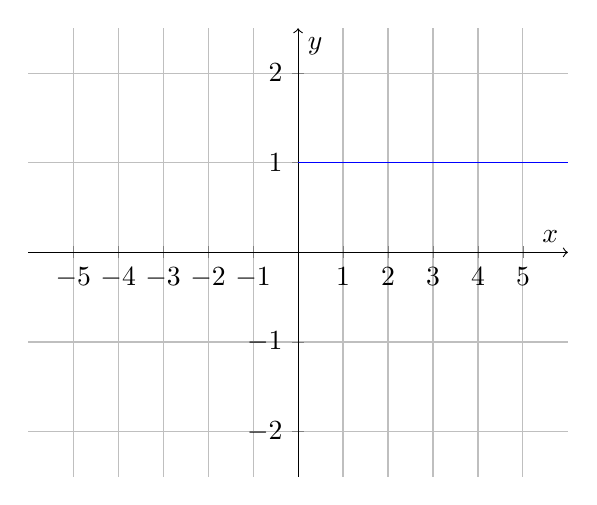
\begin{tikzpicture}
    \begin{axis}[
        xlabel={$x$},
        ylabel={$y$},
        axis lines=middle,
        axis line style={->},
        xmin=-6,
        ymin=-2.5,
        xmax=6,
        ymax=2.5,
        xtick={-5,-4,-3,-2,-1,0,1,2,3,4,5},
        ytick={-2,-1,0,1,2},
        legend style={at={(0.95,0.95)},anchor=north east},
        grid=both
      ]
        \addplot[domain=0:10, samples=100, color=blue]{1};
    \end{axis}
\end{tikzpicture} \\

\begin{equation*}
    |y| = \begin{cases}
        \;1  & x>0 \\
        \;0 & x \leq 0
    \end{cases}
\end{equation*}


discussing the concept of a "step function" in the context of neural networks and how it's used to model the behavior of neurons. Let me break it down for you:

\begin{itemize}
    \item In the brain, neurons are the basic functional units. They receive input signals from other neurons and, if the sum of those inputs reaches a certain threshold, the neuron "fires" or activates, transmitting a signal to other neurons. This activation is like turning on a switch, and it's a fundamental concept in neural activity.
    \item Step  When designing artificial neural networks (like those used in machine learning and deep learning), we often want to model the behavior of biological neurons. In this context, the "step function" is a simple mathematical function used to mimic the behavior of neurons.
    \item Think of the step function as an "on-off switch." If the input to the step function exceeds a certain threshold, the function's output is "on" (1), and if the input is below the threshold, the output is "off" (0). This behavior closely resembles the way biological neurons work, as they either fire or do not fire.
    \item The term "step" in the step function comes from the shape of its graph. When you plot this function on a graph, it looks like a step, where the output suddenly changes from 0 to 1 (or vice versa) at a specific threshold value.
\end{itemize}

In the previous function, x represents the input to the neuron, and \textbf{threshold}(whether the input is smaller or bigger than 0) is the value at which the neuron "fires." If x is less than the threshold, the output is 0 (off), and if x is greater than or equal to the threshold, the output is 1 (on).
In other words
For a step function, if the neuron’s output value, which is calculated by $sum(inputs\cdot weights)$
$+ bias$, is greater than 0, the neuron fires (so it would output a 1). Otherwise, it does not fire
and would pass along a 0. The formula for a single neuron might look something like:

 % Section 1 - Introduction

% Chapter 4 - Introduction to AI and ML %
\chapter{AI and Machine Learning}
\section{Supervised and Unsupervised Learning}

\subsection{Supervised Learning1}
Supervised learning is a type of machine learning algorithm that uses a known dataset (called the training dataset) to make predictions. The training dataset includes input data and output data. The key of supervised learning is that you give your learning algorithm examples to learn from that include the "right answers", in other words the correct label \textbf{y} for the input \textbf{x}.
It learns by seeing correct pairs of inputs and outputs.  The goal is that eventually the algorithm will only be provided with the input-value(x) and it has to predict the output-value/label(y).
Examples: \\ \\ \\

\begin{align*}
  \scalebox{1.3}{
    \begin{tabular}{|c|c|c|}
      \hline
      Input(x)          & Output(y)              & Application         \\
      \hline
      email             & spam?(0/1)             & spam filtering      \\
      \hline
      audio             & text transcript        & speech recognition  \\
      \hline
      English           & Spanish                & machine translation \\
      \hline
      ad,user,info      & click?(0/1)            & online advertising  \\
      \hline
      image, radar info & position of other cars & self-driving car    \\
      \hline
      image of a phone  & defect?(0/1)           & visual inspection   \\
      \hline
    \end{tabular}}
\end{align*}

In all of these applications you first train your model on data where you know the correct output. Then you use that model to make predictions on new data. \\

\subsubsection*{Regression: Housing Price Prediction}
Regression is a type of supervised learning algorithm that tries to predict a continuous output variable. In other words, it is used to predict a number. For example, predicting the price of a house in dollars is a regression problem whereas predicting whether a tumor is malignant or benign is a classification problem. \\
In other words, Regression is a type of algorithm that tries to predict a continuous output variable.

\subsubsection*{Classification: Breast Cancer Prediction}
Say that you are trying to create a model that predicts whether or not a tumor is malignant or benign. In classification problems, the output variable is a category (such as "malignant" or "benign"). What we are trying to do is map input variables to discrete categories, we are classifying the input values into categories and trying to predict from the two possible output. Here we have a number of possible categories or outputs that our algorithm can predict. Whereas with regression we are trying to predict a continuous number.
To summarise, Classification is a type of algorithm that tries to predict a discrete category, that doesn't necessarily have to be a number. Also in classification we are predicting a small set of possible outputs, so we are given our "options" in regards of what can our output be.
By extension obviously, we can have two or more inputs, in this case we can think of inputs as a "context" dataset that is provided to us, such as the tumor size, or the patient's age, sex, etc... The more context we provide the more accurate our prediction will be.
What we often do is represent our data-set in a function for example and our algorithm would try to identify some form of pattern in the data-set.

\subsection{Summary of Supervised Learning}
In summary supervised learning is when we are given a data-set and we are told what our correct output should be. We are given the "right answers" and we are trying to learn from that data-set to be able to predict the correct output for new data without the need of the input.
We have looked at two categories of supervised learning, regression and classification. In regression we are trying to predict a continuous number, and in classification we are trying to predict a discrete category.


\subsection{Unsupervised Learning}

Previously, in our classification problem what we have looked at is a supervised learning problem. We have a data-set and we are given the correct output(y) for each example. In unsupervised learning we are given a data-set but we are \textbf{not} given any labels or output value(y). Say you were given with the tumor size and the patient's age and any other context, however you don't know whether the tumor is malignant or benign. You are not given any labels or output value.
Our job here is not to predict whether the tumor is malignant or benign, but rather to find some structure in the data-set. In other words find something interesting in the unlabeled data-set.
The reason why it is called unsupervised is because we are not supervising the algorithm, we are not telling it what the correct answer is, we are just giving it the data and asking it to find some structure in the data.
So it might identify that the data can be divided into number of sections, or it might find some form of patterns between the patient's age and their tumor size, or any other contextual prediction.
Essentially it tries to place the data into different clusters, clustering is a type of unsupervised learning, where we are trying to find some structure in the data. For example clustering is used in google news.
What google news does is every day it goes through all the news articles that are published and it tries to group them into different clusters, so that it can show you the different clusters of news articles and you can choose which cluster you are interested in.

Another type of unsupervised learning is anomaly detection where we are trying to find some abnormal behavior in the data. For example, if we have a data-set of credit card transactions and we are trying to find some unusual behavior in the data-set, such as unusual credit card transactions.
Another example is in manufacturing, where we are trying to find some unusual behavior in the manufacturing process, such as unusual defects in the product.
We also have dimensionality reduction where we are trying to take a data-set with a large number of features and reduce the number of features to a smaller number. For example, if we have a data-set with a large number of features, we might want to reduce the number of features to a smaller number so that we can visualize the data more easily.

\subsection{Linear Regression: House sizes and prices}
In this example let's imagine that we are given with a data-set about house prices and their sizes. We are given the size of the house in square feet and the price of the house in dollars. We are given a number of examples of houses and their prices. We are trying to predict the price of a new house given its size.
This is a perfect example of a linear regression model where we would first train our model on the data-set and showing the "right answers" and then we can use that model to predict the price of a new house given its size.

A data-set that is used to train a model is called a training set. The sizes of the house can be represented with x as for example if we  have a house that is 1000 square feet, we can represent that with x = 1000. The price of the house can be represented with y, so if the price of the house is 200,000 dollars, we can represent that with y = 200,000.

We call x as the "input" variable or feature, and refer to y as the "output" variable or target.

We can represent as a single training example by $$(x,y)$$ where x is the input and y is the output.
Our $i$th training example where I would represent a specific row from the training set would look like this: $(x^{(i)},y^{(i)})$.

Note that this doesn't mean that we are taking x and y to the power of i, but rather that we are taking the i'th training example from the training set.

So for example one example would look like this $$ (x^{(1)}, y^{(1)})=(2104,400) $$

Also as mentioned $$x^{(2)}\neq x^2$$

\subsection{Process of a Supervised training}
Supervised learning algorithm will input a dataset and then what exactly does it do and what does it output?
Recall that a training set in supervised learning includes both the input features, such as the size of the house and also the output targets, such as the price of the house. The output targets are the right answers to the model we'll learn from.
To train the model, you feed the training set, both the input features and the output targets to your learning algorithm. Then your supervised learning algorithm will produce a function which we can call as $f$ that maps from x's to y's.
As every function this function will take an input x and then output a y which we can also call y-hat $\hat{y}$. So for example if we have a house that is 1000 square feet, we can input that into our function and it will output a price for that house.
y-hat in machine learning is the predicted output.
The function $f$ is called the "model". When we see only $y$ that is the actual output, when we see $\hat{y}$ that is the \textbf{predicted} output.
When designing the learning algorithm the question is that how do we choose the function $f$? What is the math formula that we are going to use?
Inspired by the \textbf{slope-intercept form} $y=mx+b$ where $m$ is the slope and $b$ is the y-intercept, we can use the following formula for our function $f$:
$$ f_{w,b}(x) = wx + b $$
For now just note that both $w$ and $b$ are real numbers and will determine the prediction $\hat{y}$
Alternatively, we don't always have to include $w$ and $b$ we can simply just write $f(x)$ and it would be the same.
We can represent the training set on a graph where our goal is to find the best fitting line using our function $f$.
We are using that function for future predictions, this process is what we call \textbf{Linear Regression with one variable} because we only have $x$ as the input which is the size of the house.
Now go through the model representation

\subsection{Cost Function}
The cost function will tell us how well the model is doing so that we can improve it and make sure that it's going to get better over time.
Recall that we have introduced our model: $$ f_{w,b}(x) = wx + b $$ and just to add a bit more terminology to it, we can call $w$ as the weights and $b$ as the bias.
Again this is what we call the slope-intercept form of a line, where $w$ is the slope and $b$ is the y-intercept.
For example if we were to have two points on a graph, let's say that we'd have the points (1,3) and (2,5) and we want to find the line that best fits these two points. We can use the slope-intercept form of a line to find the best fitting line.
First we have to find the slope, which is the change in y over the change in x, so we can calculate the slope as follows:
$$ m=\frac{\Delta x}{\Delta y}=\frac{y_2-y_1}{x_2-x_1}={\frac{5-3}{2-1}}=2 $$
Now that we have the slope we can find the y-intercept by using the following formula:
We can substitute the slope and one of the points into the formula to find the y-intercept:
$$ 3=2+b $$
$$ b=1 $$
So now we have the slope and the y-intercept, we can write the equation of the line as follows:
$$ y=2x+1 $$
Now this equation is the equation of the line that best fits the two points. We can plot the line on the graph and we can see that it fits the two points perfectly.
Obviously this was very easy and we also assumed that the line will go through these points, however this will not likely be the case in real life.
In real life we will have a lot more points and we will have to find the line that best fits all of these points. In order to do so we will have to use a cost function.
A cost function is a measure of how well a machine learning model performs by quantifying the difference between predicted and actual outputs.
In other words it will compute the difference between: $\hat{y}$ and $y$ as $\hat{y}-y$.
This difference is called the error, and we can also call it the loss.
We can also square the error to make sure that it is positive, so we can write the error as follows:
\begin{align*}
  \scalebox{1.3}{$
    \sum_{i=0}^{m}\ (\hat{y}^{(i)}-y^{(i)})^2
  $}
\end{align*}
This case $m$ is the number of training examples, so we are summing over all of the training examples.
The problem here is that the more training examples we have, the larger the error will be. So we will have to divide the error by the number of training examples in order to avoid this huge numbers, so we can write the error as follows:
\begin{align*}
  \scalebox{1.3}{$
    \frac{1}{m}\sum_{i=0}^{m}\ (\hat{y}^{(i)}-y^{(i)})^2
  $}
\end{align*}

By convention machine learning people used to divide by $2m$, and also we can refer to the cost function as $J_(w,b)$ so our overall cost function will look like this:
\begin{align*}
  \scalebox{1.3}{$
    J_{(w,b)}=\frac{1}{2m}\sum_{i=0}^{m}\ (\hat{y}^{(i)}-y^{(i)})^2
  $}
\end{align*}

This is what we call the squared error cost function that is being used most commonly.

Now make sure to be aware of this:
\begin{align*}
  \scalebox{1.3}{$
    J_{(w,b)}=\frac{1}{2m}\sum_{i=0}^{m}\ (f_w,b(x^{(i)})-y^{(i)})^2
  $}
\end{align*}

\subsection{More deeply about cost function}
We will use one example and actually get to see how the cost function can be used to find the best fitting line.
Now let's recap what we have so far.
\begin{enumerate}
  \item \textbf{model:} We have our \textbf{model} which is represented with the slope-interecept function: $f_w,b(x)=wx+b$ and depending on what values we choose for the slope $w$ and the y-interecept $b$ we are getting a line.
  \item  \textbf{parameters:} The model's parameters will $w$ and $b$, again our goal is to find the best values for $w$ $b$ to get the best fitting lines.
  \item \textbf{cost function:} Now in order to measure how good the values for $w$ and $b$ are we are using our cost function which we have constructed before: $$ J_{(w,b)}=\frac{1}{2m}\sum_{i=0}^{m}\ (f_w,b(x^{(i)})-y^{(i)})^2 $$
        We are taking the difference between the predicted value and the actual value for $y$, so we are trying to reduce the value of $J$
  \item \textbf{goal: } So we can say that our goal is to: $$ minimize J(w,b)$$
\end{enumerate}

Now let's see an example of how the cost function and the model would work.
For simplicity we can get rid of the y-intercept $b$ meaning that our graphs will pass through the origin.

\begin{align*}
  \includegraphics[width=1.2\textwidth]{machine-learning/andrew_ng_intro_to_ml/cost_function.png}
\end{align*}

As you can see here we have started off by plotting 3 points in which were: $(1,1)$ $(2,2)$ and $(3,3)$
Then what we wanted to do is test out our const function. We have identified the slope $w$ to be $1$ which ended up passing through all of the points perfectly.
Since this line passes through all of the points we expected $J(x)$ to be 0. \\
Notice that when evaluating $J$ we are passing in the slope $w$ as the parameter.
As you can see we have evaluated $J(w)$ and as we expected it turned out to be 0.
In the other graph we can see that if we visualise the our slopes and const function solutions in a graph where we have the axis $w$ and $J(x)$.
We can see that when $w=1$ $J(x)=0$.
The reason why the cost function is zero, is because we have identified the slope of the function successfully which resulted the \textbf{perfectly} fitting line.
We can validate our slope calculation by this formula: $$ m=\frac{\Delta y}{\Delta x}=\frac{1}{1}=1 $$ In short the slope is just a fraction of the change in y over the change in x.

Now let's try a different value of $w$ and pretend that we wouldn't know how to calculate the slope of this line.
If $w=0.5$ then obviously it's not going to fit the points well, therefore we expect $J(x)$ to be more than 0.

\begin{align*}
  \includegraphics[width=1.2\textwidth]{machine-learning/andrew_ng_intro_to_ml/cost_function_0.5.png}
\end{align*}

We can see here that the line doesn't fit well to the points, therefore when calculating the difference between $\hat{y}-y$ and then square it we are actually going to get a number bigger than 0.
We can see that what we actually count by the difference $\hat{y}-y$ is the height from the predicted value to the actual value.
When $w=0$ this is how it would look:

\begin{align*}
  \includegraphics[width=1.2\textwidth]{machine-learning/andrew_ng_intro_to_ml/cost_function_0.png}
\end{align*}

We see that in this case since the slope of the line is $0$ and it has a y-intercept of 0, it's just going through the x-axis.
Obviosuly we could have had negative values for $w$ and then the cost function would have ended up being more, but in conclusion the further is the distance between the predicted and actual values the more the cost function is going to be.
If we keep going with the values we can see that the graph between $w$ and $J(w)$ turns out to be a curve.

\begin{align*}
  \includegraphics[width=1.2\textwidth]{machine-learning/andrew_ng_intro_to_ml/cost_function_slope_curve.png}
\end{align*}

This curve shows the different values of the cost function with their slopes.
As we can see our goal was to have the smallest value of $J(w)$ and by our equation we concluded that when $J(w)=0$ will be $w=1$ which can be perfectly seen in the graph.

This is how you can use the cost function to identify the best fitting slope $w$.
Obviosuly we could have gotten further by having the y-intercept $b$ as a parameter but let's leave that to the next sections.

In summary, we have conducted that the goal of linear regression is to choose values for $w$ and $b$ that results the cost function $J$ to be the smallest value possible.
In order to find the best values for $w$ and $b$ we have to introduce the idea of gradient descent

\subsection{Gradient Descent}
Obviosuly our goal would be to find a systematic way of finding values for $w$ and $b$ that fits the data perfectly or results with the smallest possible cost $J$.
Gradient descent (GD) is an iterative first-order optimisation algorithm, used to find a local minimum/maximum of a given function. This method is commonly used in machine learning (ML) and deep learning (DL) to minimise a cost/loss function (e.g. in a linear regression).
Here is an overview of what we would want to achieve:
\begin{itemize}
  \item We have the function $J(w,b)$, gradient descent can be used to minimize not just the cost function but any given function.
  \item Our goal is to minimize it as min $J(w,b)$
  \item \textbf{Outline: } So this is how it works:
        \begin{enumerate}
          \item Start with some initial guesses for $w$ and $b$, it wouldn't matter that what would you start off with but it's a convention to start off with both $w=0$ and $b=0$
          \item Then what you will do is you will keep changing $w,b$ to reduce $J(w,b)$
          \item Until we settle at or near a local minimum which may be more than 1.
        \end{enumerate}
\end{itemize}

\subsection{Gradient Descent Mathematically}
So this is how it looks:
$$\displaystyle w=w-\alpha \frac{d}{dw}J(w,b) $$
Let's unpack the details of this equation. \\
First the equal notation $=$ in this case is an assignment operator. So we are going to take the value of $w-\alpha \frac{d}{dw}J(w,b)$ and store it in the variable $w$, this is thinking programatically
Because if we think matematically we claim that $w$ is equal to $w-\alpha \frac{d}{dw}J(w,b)$ which is not true, we are storing the value of $w-\alpha \frac{d}{dw}J(w,b)$ in the variable $w$. In conclusion the equal sign can be used for either assignment or truth assertion.
Let's unpack the different symbols in this equation:
\begin{itemize}
  \item $\alpha$ which is a greek letter, in this case the alpha is the \textbf{learning rate} which is a very small positive number such as 0.01, 0.001, 0.0001, between 0-1.
        $\alpha$ will determine how big of a step we take downhill on each iteration. By extension if its relatively big then we will take a big step downhill, if it's relatively small then we will take a small step downhill.
        Downhill means that we are trying to reduce the value of $J(w,b)$.
        We will go deeper in terms of choosing a good value for $\alpha$
  \item $\frac{d}{dw}J(w,b)$ is the derivative of the cost function $J(w,b)$ with respect to $w$. However we are going to talk about this in much more detail. You can think of the derivative as the direction and magnitude of the steps.
\end{itemize}

You have another parameter which is $b$ and you can update it in a similar way:
$$\displaystyle b=b-\alpha \frac{d}{db}J(w,b) $$

As a detail you want to make sure that you are updating $w$ and $b$ simultaneously, meaning that you want to update them at the same time. Also you are updating them from their old values, so you are not updating $w$ and $b$ from the original values but rather from their old values.


Here is the correct and incorrect way of updating $w$ and $b$:
\begin{align*}
  \includegraphics[width=1\textwidth]{machine-learning/andrew_ng_intro_to_ml/gradient_descent_implementation.png}
\end{align*}
\subsection{More deeply about gradient descent}
so here is the gradient descent algorithm:
$$ w=w-\alpha \frac{\partial L}{\partial w}$$
where $\alpha$ is the learning rate, and $\frac{\partial L}{\partial w}$  is the derivative term
and also for b:
$$ b=b-\alpha \frac{\partial}{\partial w}$$
where $\frac{\partial}{\partial b}$ is the derivative term \\

Just for the sake of simplicity let's assume that we are only dealing with $w$ and not $b$.
So our cost function would turn into $J(x)$ and our algorithm would change into:
$$ w=w-\alpha \frac{\partial J}{\partial w}$$

Let's look and talk about this diagram:
\begin{align*}
  \includegraphics[width=1\textwidth]{machine-learning/andrew_ng_intro_to_ml/gradient_descent_visualisation.png}
\end{align*}

Now as a remainder our goal is to find the $w$ where the $J(x)$ is the smallest. Gradient descent helps us find the local minimum of the cost function $J(x)$.
Looking at the first example we have started off with a random example then what the derivative does is it uses something called the tangent line to find the slope of the line at that point.
The tangent line is a line that touches the curve at that point. As we can see we are getting back 2 which means that it is a positive number.
We know that the learning rate $\alpha$ is a positive number, so looking into the subtraction its obvious that we are going to reduce the value of $w$.
By extension we are going backwards which proves the gradient descent functionality as we are getting closer to the local minimum.
Now let's look at the second example where we are getting a negative number and when we subtract a negative number we essentially are adding a positive number which is going to increase the value of $w$, so we are going to go forward, which again proves the gradient descent as we are getting closer to the local minimum.

In summary the derivative term will use the tangent line to find the slope of the curve at a given point, then we use that slope to find the direction of the step that gets us closer to the local minimum. Now the last thing that we don't really understand is the learning rate $\alpha$.

\subsection{Learning rate}
The value of $\alpha$ has a huge impact on the efficiency of the gradient descent. If it is chosen poorly then the gradient descent might not work at all.

To understand the impact and the significance of the learning rate let's look at what happens when it's either too big or when it's too small.

\begin{align*}
  \includegraphics[width=1\textwidth]{machine-learning/andrew_ng_intro_to_ml/learning_rate_big_small.png}
\end{align*}

Now if the learning rate is too small then the gradient descent will take a long time to converge, meaning that it will take a long time to find the local minimum.
However we will still find the minimum, it will just take a long time.
When the learning rate is too big then the gradient descent might not converge at all, meaning that it might not find the local minimum. This can happen when the learning rate is too big and it goes over the local minimum and it stucks in a loop.

Now one thing to mention is what happens when the gradient descent reaches the local minimum.
Let's look at this diagram:
\begin{align*}
  \includegraphics[width=1\textwidth]{machine-learning/andrew_ng_intro_to_ml/local_minimum_validation.png}
\end{align*}

As you can see when the gradient descent reaches the local minimum the derivative will be 0, so when we multiply it by the learning rate $\alpha$ it will be 0, and when subtractng 0 from $w$ it will be the same value.
In conclusion when we reach a local minimum further gradient descent steps will do absolutely nothing, so we can stop the gradient descent when we reach a local minimum.

Let's look at another concept that how gradient descent can reac local minimum with fixed learning rate.
\begin{align*}
  \includegraphics[width=1\textwidth]{machine-learning/andrew_ng_intro_to_ml/local_minimum_fixed_learning_rate.png}
\end{align*}

As we can see when we take the first step, the slope of the tangent line at that point is really big, therefore we are taking a big step.
As we are taking the steps the slope of the tangent line is getting smaller and smaller, therefore we are taking smaller and smaller steps.
When we reach the local minimum the slope of the tangent line is 0, therefore we are not taking any steps.
This explains that whenever we are approaching the local minimum the steps are getting smaller and smaller, because the slope is smaller, then the derivative is smaller and $w$ is smaller so we are taking a smaller step.
In conclusion the gradient descent can reach the local minimum without decreasing the learning rate $\alpha$.

\subsection{Put it all together - Gradient Descent for Linear Regression}
Now let's put it all together and see how we can use gradient descent to find the best fitting line for our data-set.
Recall that we have the following model: $$ f_{w,b}(x) = wx + b $$
We have the following cost function: $$ J_{(w,b)}=\frac{1}{2m}\sum_{i=0}^{m}\ (f_w,b(x^{(i)})-y^{(i)})^2 $$
And we have the following gradient descent algorithm:
$$ w=w-\alpha \frac{\partial}{\partial w}J(w,b)$$
$$ b=b-\alpha \frac{\partial}{\partial b}J(w,b)$$


\subsection{Calculate the derivative terms}

We have this derivative with respect to $w$:
$$ \frac{\partial}{\partial w}J(w,b)$$
We start by plugging in the definition of $J(w,b)$:
$$ \frac{\partial}{\partial w}J(w,b)=\frac{\partial}{\partial w}\frac{1}{2m}\sum_{i=0}^{m}\ (f_w,b(x^{(i)})-y^{(i)})^2$$
Remember that $f_w,b(x^{(i)})$ is the same as $wx^{(i)}+b$ so we can substitute that in:
$$ \frac{\partial}{\partial w}J(w,b)=\frac{\partial}{\partial w}\frac{1}{2m}\sum_{i=0}^{m}\ (wx^{(i)}+b-y^{(i)})^2$$
We know that the derivative is equal to will be equal to $2x^{(i)}$ so we can substitute that in:
$$ \frac{\partial}{\partial w}J(w,b)=\frac{1}{m}\sum_{i=0}^{m}\ (wx^{(i)}+b-y^{(i)})x^{(i)}$$
Let's do the same thing for $b$:
$$ \frac{\partial}{\partial b}J(w,b)=\frac{\partial}{\partial b}\frac{1}{2m}\sum_{i=0}^{m}\ (f_w,b(x^{(i)})-y^{(i)})^2$$
and we can substitute $f_w,b(x^{(i)})$ with $wx^{(i)}+b$:
$$ \frac{\partial}{\partial b}J(w,b)=\frac{\partial}{\partial b}\frac{1}{2m}\sum_{i=0}^{m}\ (wx^{(i)}+b-y^{(i)})^2$$
We know that the derivative is equal to will be equal to $2$ so we can substitute that in:
$$ \frac{\partial}{\partial b}J(w,b)=\frac{1}{m}\sum_{i=0}^{m}\ (wx^{(i)}+b-y^{(i)})$$

Now that we know this we can apply them to the gradient descent algorithm:
repeat until convergence \{
$$ w=w-\alpha \frac{1}{m}\sum_{i=0}^{m}\ (wx^{(i)}+b-y^{(i)})x^{(i)}$$
$$ b=b-\alpha \frac{1}{m}\sum_{i=0}^{m}\ (wx^{(i)}+b-y^{(i)})$$
\}

The model representation shows how these algorithms are made up in code.

\subsection{Multiple Features}

So far we have only looked at the case where we have one input feature, such as the size of the house. However in real life we will have multiple input features, such as the size of the house, the number of bedrooms, the number of floors, etc...
\begin{align*}
  \includegraphics[width=1.1\textwidth]{machine-learning/andrew_ng_intro_to_ml/multiple_features.png}
\end{align*}
In the original version of linear regression, you had a single feature x, the size of the house and you're able to predict y, 
the price of the house. The model was fwb of x equals wx plus b. But now, what if you did not only have the size of the house as a 
feature with which to try to predict the price, but if you also knew the number of bedrooms, the number of floors and the age of the 
home in years. It seems like this would give you a lot more information with which to predict the price. To introduce a little bit of
 new notation, we're going to use the variables $X_1, X_2, X_3 and X_4$, to denote the four features. For simplicity, let's introduce 
 a little bit more notation. We'll write X subscript j or sometimes I'll just say for short, X sub j, to represent the list of 
 features. Here, j will go from one to four, because we have four features. I'm going to use lowercase n to denote the total number 
 of features, so in this example, n is equal to 4. As before, we'll use X superscript i to denote the ith training example. 
 Here X superscript i is actually going to be a list of four numbers, or sometimes we'll call this a vector that includes all the 
 features of the ith training example. As a concrete example, X superscript in parentheses 2, will be a vector of the features for 
 the second training example, so it will equal to this 1416, 3, 2 and 40 and technically, I'm writing these numbers in a row, so 
 sometimes this is called a row vector rather than a column vector. But if you don't know what the difference is, don't worry about 
 it, it's not that important for this purpose. To refer to a specific feature in the ith training example, I will write X superscript 
 i, subscript j, so for example, X superscript 2 subscript 3 will be the value of the third feature, that is the number of floors in 
 the second training example and so that's going to be equal to 2. Sometimes in order to emphasize that this$X^2$ is not a number but 
 is actually a list of numbers that is a vector, we'll draw an arrow on top of that just to visually 
 show that is a vector and over here as well, but you don't have to draw this arrow in your notation. 
 You can think of the arrow as an optional signifier. They're sometimes used just to emphasize that this is a vector 
 and not a number. Now that we have multiple features, let's take a look at what a model would look like.

 \begin{align*}
  \includegraphics[width=1.1\textwidth]{machine-learning/andrew_ng_intro_to_ml/model_representation.png}
\end{align*}

The definition of model with n features is going to be $f_w,b(x)=w_1x_1+w_2x_2+...+w_nx_n+b$.
We can make this easier by defining $w$ as a vector: 
$$\vec{w}=[w_1,w_2,...,w_n]$$
$w$ and $b$ are the parameters of the model. 
We can also define $x$ as a vector:
$$\vec{x}=[x_1,x_2,...,x_n]$$

Therefore we can rewrite the model as follows:
$$f_w,b(\vec{x})=\vec{w}\cdot\vec{x}+b$$
where $\vec{w}\cdot\vec{x}$ is the dot product of the two vectors.
A linear regression with multiple features is called a multiple linear regression.

\subsection{Gradient Descent for Multiple Features}

Now let's look at how we can use gradient descent for multiple features.
\begin{align*}
  \includegraphics[width=1.1\textwidth]{machine-learning/andrew_ng_intro_to_ml/gradient_descent_multiple_regression.png}
\end{align*} \break % Section 1 - Supervised and Unsupervised Learning

\chapter{Discrete Mathematics}
\section{Mathematical thinking}
\section{Variables}
A variable is sometiems thought of as a mathematical "John Doe" because you can use it as a placeholder when you want to talk about 
something but either you imagine that it has one or more values but you don't know what they are, or you want whatever you say
about it to be equally true for all elements in a given set. This can be easily recognised/understood in programming languages where variables play a vital role and 
fundemental part of the language. It has slighly different meanings in mathematics and computer science. When one uses variable in mathematical terminology it can be defined
as a symbol that represents a quantitiy in a mathematical expresssion, as used in many sciences. In computer science it is rather something storying a value and this associated value may be changed(mutable).


\section{Mathematical statements}
Three of the most important kinds of sentences in mathematics are universal statements, conditional statements, and existential statements.

\textbf{Universal statement}: A universal statement says that a certain property is true for all elements in a set. 
\textbf{Conditional statement}: A conditional statemetn says that if one thing is true then some other thing also has to be true.
\textbf{Existential statement}:   An existential statement says that there is at least one thing for which the propert is true.


In other words,
\textbf{Universal statement}
\textbf{Conditional statement}
\textbf{Existential statement}:
\end{document}

